% !TEX root = ../thesis.tex
\chapter{Konstrukce ASR systému pro uživatele po totální laryngektomii hovořící pomocí elektrolarynxu}
\label{chap:construction}


% V předchozích sekcích bylo zmíněno, že velmi významný problém představuje psychologický faktor ztráty hlasu. Ten sebou nese i na první pohled néúplně zřejmou komplikaci. A tou je obtížnost získávání řečníků po TL, kteří jsou ochotní spolupracovat na výzkumu.

% Jedním z možných řešení je, že se výzkumníci sami naučí používat jednu z výše  \todo{TBD}{[c4l1]})zmíněných metod produkce řeči. Pro účely našeho výzkumu a rámec této práce by se jednalo o elektrolarynx. I když se tato možnost jeví poměrně jednoduše, tak zdání klame. Přestože je zdravý řečník schopen obstojně mluvit (pomocí EL), za relativně krátkou dobu tak k tomu, aby produkovaná řeč svými parametry odpovídala zkušenému řečníkovi po TL, je potřeba relativně dlouhá doba.ě

% V našem případě se podařilo získat pouze jednoho zkušeného řečníka\footnote{Jedná se o ženu v důchodovém věku, která ale stále působí na akademické půdě a jednou za čas i přednáší.}, který podstoupil TL před více než 15 lety a EL používá aktivně každý den. Je to jeho jediná možnost jak produkovat slyšitelnou řeč.

% Díky spolupráci s tímto řečníkem jsme byli schopni získat cca 15 hodin promluv (více o získaných datech v \ref{chap:experiments:analysis} a \ref{chap:experiments:normalization}), které byly použity pro všechny dosavadní experimenty. Z pohledu standardních obecných systémů rozpoznávání řeči se to může jevit jako velmi malé množství, ale jak ukáží následné experimenty, tak to není velký problém. Jelikož už před prvními experimenty se jevilo jako prozaičtější vytvářet individuální modely pro každého řečníka a výsledky experimentů toto jen podpořily.

% Při rozhovorech s řečníkem se potvrdil psychický aspekt ztráty hlasu na člověka po TL. Konkrétní osoba ještě dlouhá léta po operaci nebyla schopna telefonovat, natož mluvit na veřejnosti. Kvalita života se tímto velmi snížila a trvalo prý velmi dlouho dobu, než se daná osoba odvážila i jen odpovědět na nečekaný telefonní hovor. To pro nás představovalo nezanedbatelnou porci motivace v práci.

% V následujícím textu si přiblížime a zanalyzujeme pořízená data (\ref{chap:experiments:analysis}) a na základě těchto prvotních experimentů nadefinujeme cíle a určíme další postup. V části (\ref{chap:experiments:normalization}) si popíšeme normalizaci dat a porovnáme schopnosti člověka a stroje. V sekci \ref{chap:realisation:augmentation} rozebereme prvotní ověřovací experimenty s upravenými daty a v sekci \ref{chap:experiments:durationmodels} představíme výsledky modelů zohledňujících i délku fónému.

% Při konzultacích s pacienty vyšlo najevo, že psychická stránka je velmi důležitá a někdy to může věst až k paralýze (v obrazném slova smyslu) kdy ti lidé nebyli schopni třeba telefonovat. Takže systém, který by sice neřešil kompletní problematiku náhrady/rehabilitace řeči by mohl být užitečný.

% !TEX root = ../../autoreferat.tex
\section{Vytvoření řečového korpusu EL promluv}
\label{chap:construction:corpus}

% Před započetím prací na vytvoření ASR systému pracujícího s~lidmi po TL je potřeba vytvořit řečový korpus, který poslouží  k~natrénování a otestování vytvořeného systému. Tato data jsou velmi specifická. Proto je potřeba zajistit co možná největší množství kvalitních\footnote{Kvalitou je myšlena věrnost dat dané doméně, dále se mluví o přesnosti ve smyslu bezchybnosti přepisů.} a přesných dat, která budou součástí řečového korpusu.

% Jak už bylo zmíněno v~části \ref{chap:cause:desease}, ročně se objeví více než 100 nových případů trvalé ztráty hlasu, přičemž rizikovou skupinou osob jsou starší lidé, kteří intenzivně kouří a konzumují alkohol. Přesto je patrný trend snižujícího se věku pacientů a s~tím související nárůst případů ztráty hlasu. Přičteme-li již výše zmíněný psychologický aspekt jeho ztráty, je zřejmé, jak komplikované je zajistit spolupráci byť s~jediným řečníkem ochotným podstoupit náročné\footnote{I pro zdravého člověka je někdy několikahodinové nahrávání vysilující. Pro jedince po TL to je z mnoha důvodů ještě řádově náročnější.} nahrávání.

% Proto došlo  k~navázání kontaktů se specializovanými pracovišti ORL, v~našem případě byly nejprve navázány kontakty s~ORL klinikou při Fakultní nemocnici v~Plzni, a následně i s~ORL klinikou Fakultní nemocnice v~Motole.
S pomocí lékařů ORL kliniky při Fakultní nemocnici v~Plzni byla navázána spolupráce s~jedním řečníkem, konkrétně se jedná o dámu v~důchodovém věku, která podstoupila TL před více než 15 lety.
% Po překonání ostychu\footnote{Podle jejích vlastních slov nebyla schopna několik let po operaci ani zvednout nečekaný telefonní hovor, natož mluvit na veřejnosti.} se byla schopna naplno vrátit do běžného života a dokonce v~určité formě opět přednášet o stomatologii na Lékařské fakultě v~Plzni, Univerzity Karlovy.
S její pomocí bylo na pracovišti Katedry kybernetiky ZČU v~1.~etapě nahrávání,
% v~období od prosince 2010 do května 2011,
pořízeno více než 10 hodin promluv.
% během 14 samostatných sezení více než 10 hodin promluv, viz tab. \ref{tab:construction:recording}.
% Každé sezení trvalo přibližně dvě hodiny a bylo rozděleno na fáze nahrávání a fáze odpočinku. Fáze nahrávání trvaly 10 - 20 minut.
Pořízené dílčí nahrávky obsahují několik vět, které jsou vzájemně odděleny úseky ticha o minimální délce 5~s.
% Fáze odpočinku mezi nahráváním dílčích segmentů trvaly přibližně 10 minut.
% Bylo nezbytné je do harmonogramu zařadit zejména z~důvodu únavy řečníka.
Získaná data neobsahují žádný nežádoucí ruch kromě samotného zvuku EL i přesto, že nahrávání neprobíhalo v~profesionálním studiu.

% \begin{table}[htpb]
%   \centering
%   \def\arraystretch{1.5}
%   \pgfplotstabletypeset[
%     col sep=comma,
%     string type,
%     columns/phase/.style={column name={Nahrávání}, column type={l}},
%     columns/length/.style={column name={Délka \textit{[HH:MM:SS]}}, column type={r}},
%     columns/sentences/.style={column name={Počet vět}, column type={r}},
%     columns/files/.style={column name={Počet souborů}, column type={r}},
%     every head row/.style={
%       after row={
%         \cmidrule(r){1-1}
%         \cmidrule(lr){2-2}
%         \cmidrule(lr){3-3}
%         \cmidrule(l){4-4}
%       },
%       before row={\toprule}
%     },
%     every last row/.style={after row={\bottomrule}},
%   ]{./parts/ch5-construction/tabs/02-recording1-stats.csv}
%   \caption{Informace o korpusu nahrávek z 1. etapy nahrávání.}
%   \label{tab:construction:recording}
% \end{table}

Pro pořízení záznamů byla navržena nahrávací sestava složená z miniaturního profesionálního mikrofonu (DPA d:screet 4061-FM), zesilovače (DPA MMA6000), externí zvukové karty a běžného notebooku. Mikrofon byl pomocí bezpolštářkové náplasti přilepen co nejblíže (do bezprostřední blízkosti) pravého koutku úst mluvčí tak, aby zaznamenaná řeč měla co možná nejvyšší kvalitu.

Před samotným nahrávánám byly z databáze obsahující stovky tisíc vět pečlivě vybrány, postupem popsaným v~\cite{Radova2000}, konkrétní věty a z nich vytvořeny 2 sady vět, konkrétně:

\begin{enumerate}
  \item sada obsahující všechny fonémy vyskytující se v~češtině - \textit{40 vět};
  \item sada obsahující věty s~reálnou četností fonémů - \textit{5000 vět}.
\end{enumerate}

% \noindent Nahrané soubory vždy obsahují několik vět vzájemně oddělených minimálně 5 sekundovými úseky ticha.
% Nahrávky mouhou navíc obsahovat opakování chybně vyslovených vět, přeřeknutí, kýchnutí a další neřečové události.
% Z tohoto důvodu bylo nezbytné nahrávky rozčlenit na kratší úseky a anotovat, přestože byly pořízené na základě připravené sady vět.

Každá nahrávka je automaticky rozdělena na mikrosegmenty o konzistentní době trvání. Empiricky byla stanovena vhodná délka trvání v~rozsahu 10 - 100 ms. S~využitím metody voice activity detection (VAD) byla pro každou nahrávku stanovena hodnota energie dle vztahu

\begin{equation}
  \label{eq:construction:energy}
  E_{RMS}(n) = \sqrt{\frac{1}{N} \sum_{n=1}^{N} \left| x(n) \right|^2},
\end{equation}

\noindent kde $N$ představuje počet vzorků v~nahrávce a $x(n)$ představuje pravoúhlé okénko vzorku $n$ a následně určena průměrná energie nahrávky jako střední hodnota energií všech mikrosegmentů.
Její hodnota slouží pro nalezení úseků ticha, tj. míst, kde začíná a končí věta.
Pokud energie nějakého úseku $x$ je $E_{RMS}(x) < avg(E_{RMS})$ a zároveň délka tohoto úseku $dur(x) \geq 1\ s$, tak je možné nahrávku v~tomto úseku rozdělit.
% Na začátku a konci každého úseku je vhodné mít minimálně $0.5\ s$ ticha, aby byla zajištěna správná funkce ASR systému, viz \ref{chap:asr:parametrization}.
Na obr. \ref{fig:construction:el_speech} je zobrazena ukázka charakteru audio signálu a spektrogram promluvy \textit{\uv{Akcie Komerční banky}}.
% Zároveň jsou zde vyneseny vypočtené hodnoty energie a celková průměrná energie.
% Pokud řečník v~průběhu věty z~libovolného důvodu udělal pauzu větší než $1\ s$, tak i tato věta byla v~důsledku výše popsaného postupu rozdělena na dvě části.
% Nejedná se však o významný problém, protože při vytváření ASR systému není podstatné, zda promluva představuje celou větu, ale spíše to, zda je tento úsek správně přepsán.
% Fakt, že některé věty jsou rozděleny na více částí, je důvodem, proč v~tab. \ref{tab:construction:recording} neodpovídá počet soubourů počtu vět.

\begin{figure}[hbpt]
  \centering
  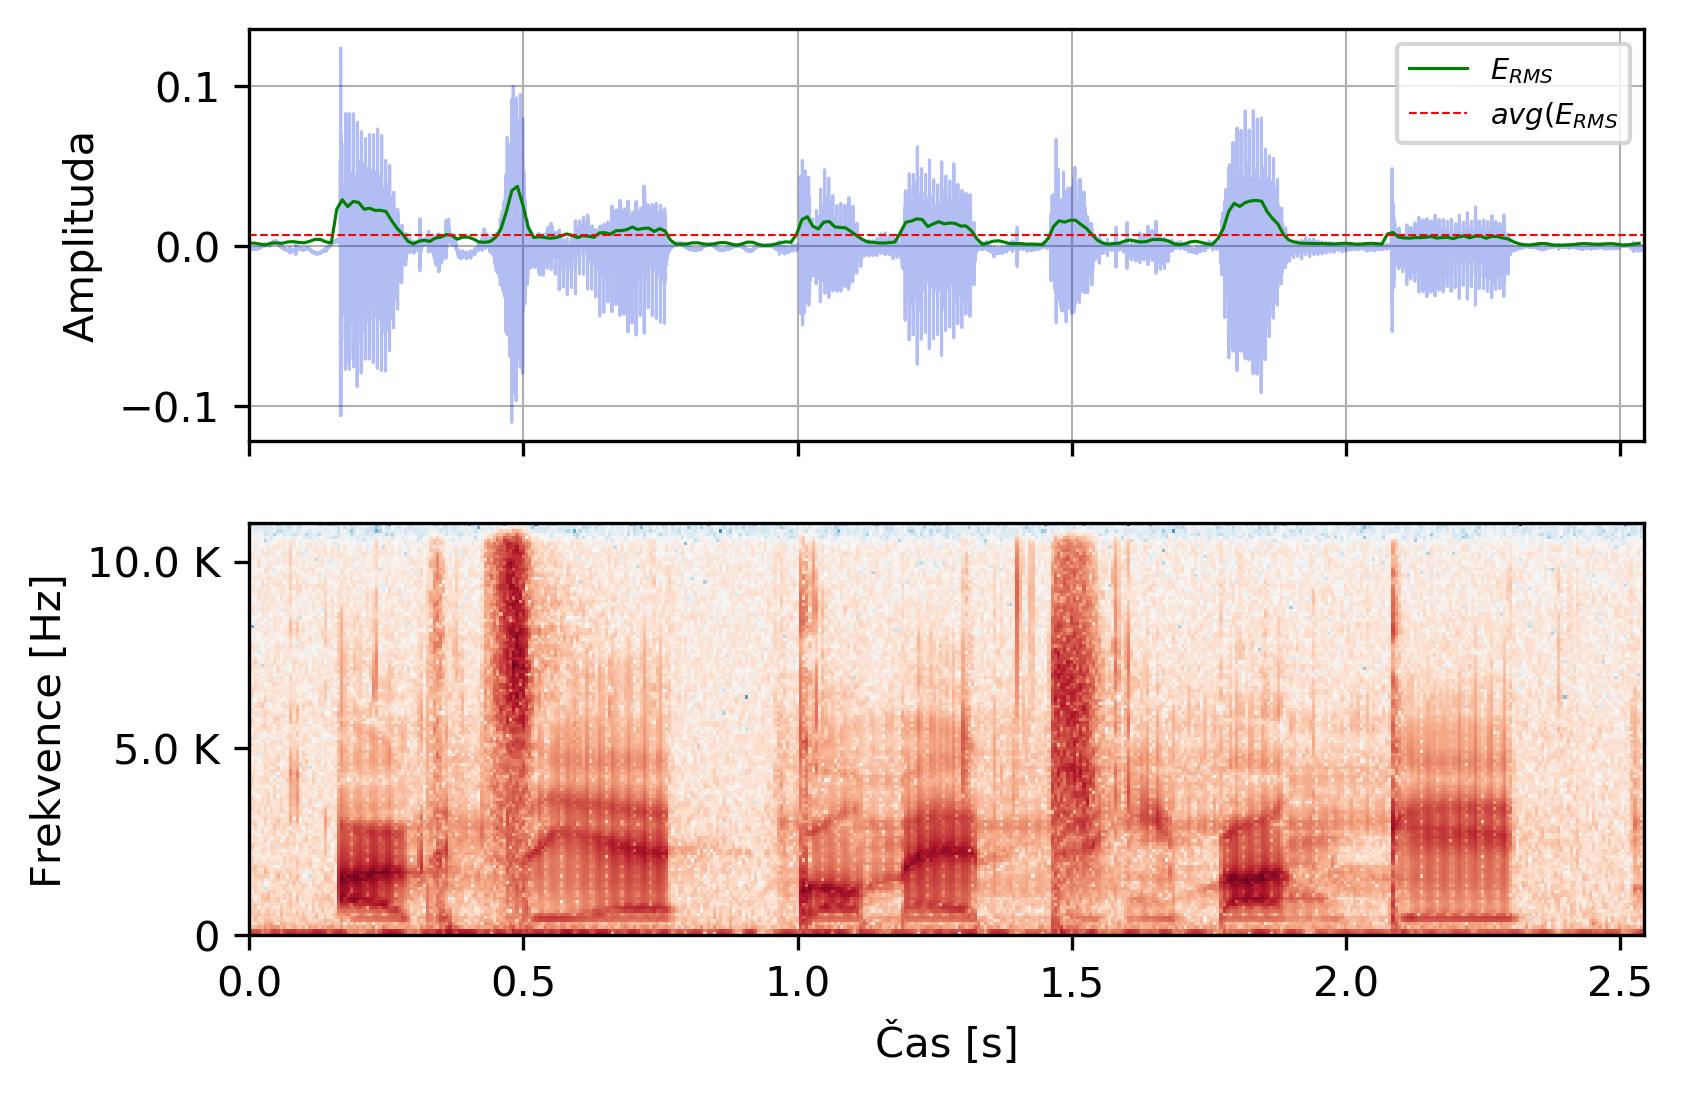
\includegraphics[width=0.9\textwidth]{./parts/ch5-construction/img/energy_spec_el.png}
  \caption[Průběh a spektrogram EL promluvy.]{Průběh a spektrogram promluvy a vyznačenou energií EL promluvy.}
  \label{fig:construction:el_speech}
\end{figure}

% K anotaci posloužil interní anotační nástroj, podíleli se na ní celkem 3 anotátoři z~řad studentů.
% Přepis každého anotátora byl vždy zkontrolován jiným anotátorem.
% Ačkoli bylo potřeba přepsat relativně malé množství dat (cca 10 hodin audio záznamu), tak anotace všech promluv trvala přibližně 2 měsíce.
% Hlavním důvodem byla relativně dlouhá doba, po kterou se anotátoři adaptovali na specifika EL řeči.
% Hlavně ze začátku nebyli schopni porozumět obsahu promluvy, a tím pádem jej správně přepsat.
% To významně prodloužilo dobu potřebnou  k~anotaci celého řečového korpusu.

% Pokud je  k~produkci řeči použit elektrolarynx, je vedlejším produktem nezanedbatelný ruch způsobený samotným zařízením, viz část \ref{chap:cause:treatment:foniatric}.
% Z~tohoto důvodu byly v~průběhu anotace ignorovány v~podstatě všechny skupiny neřečových událostí, protože vetšina nahrávek by dle pravidel anotování běžné řeči obsahovala šum.
% Výsledný řečový korpus se skládá z $5040$ unikátních vět rozdělených do $6385$ souborů (viz tab. \ref{tab:construction:recording}), které v~průměru obsahují $7$ slov o průměrné délce $5$ znaků. Tento korpus slouží jako základ pro všechny budoucí experimenty.

% !TEX root = ../thesis.tex
\section{Analýza akustického signálu a jeho parametrizace}
\label{chap:construction:analysis}

Rozpoznávání řeči se věnuje nemalé usílí již od 50. let 20. století a v současné době nikoho nepřekvapí téměř bezchybně fungující obecný rozpoznávač souvislé řeči v mobilních zařízeních. Pro obecné systémy dokonce existují korpusy s desítkami,stovkami i více hodin promluv, které je možné využít při vytváření těchto systémů.

Tyto korpusy však obsahují, ve většině případů, pouze \uv{standardní}\footnote{Slovením spojením \uv{standardní řeč} je myšlena řeč neobsahující vyrazné řečové vady, případně jiné formy produkce a často v nepřílíš akusticky náročném prostředí.} řeč. Pokud je snaha vytvořit nebo ověřit funkčnost systému za specifických podmínek (ať už se jedná o rušné prostředí či speciální typy promluv), tak je nezbytné získat potřebná data, viz \ref{chap:construction:corpus}.

\subsection{Analýza získaných dat}
\label{chap:construction:analysis:data}

Získaný korpus obsahuje přes 10 hodin akustických záznamů promluv a více či méně přesných přepisů\footnote{I přes nemalou snahu a několikastupňovou kontrolu, je téměř jisté, že by nebylo obtížné najít přepis, který obsahuje chybu například ve formě překlepu.}. V momentě kdy jsou k dispozici data je možné se podívat na specifika EL řeči a případně porovnat se zdravým řečníkem.

Pro potřeby porovnání byl použit začátek promluvy \textit{\uv{Akcie Komerční banky...}}. Tato promluva je součástí standardní množiny vět používaných při vytváření řečových korpusů na KKY při ZČU. Tím pádem je k dispozici v relativně velkém množství příkladů pro zdravé řečníky. Tato věta je součástí také korpusu EL řeči.

Na obr. \ref{fig:construction:analysis:comparison} je zobrazen průběh amplitudy a spektrogram vybrané promluvy pro zdravého (obr. \ref{fig:construction:analysis:comparison:normal}) a EL (obr. \ref{fig:construction:analysis:comparison:el}) řečníka. Už na první pohled je možné zaznamenat určité rozdíly i přesto, že obsah obou promluv je identický. Prvním takovým je délka promluvy. V případě zdravého řečníka je v průměru\footnote{Vypočteno na základě 10 náhodně vybraných promluv ze standardně používaného korpusu na katedře kybernetiky ZČU.} o celou $1$ vteřinu kratší než v případě EL řeči. Tempo řeči je samozřejmě velmi individuální, ale z principu je EL řeč pomalejší. Z průběhu signálu na obr. \ref{fig:construction:analysis:comparison:el} je patrné, že řečník dělá výraznější pauzy mezi jednotlivými slovy promluvy. Toje často způsobené potřebou naplnit jícen vzduchem. Po TL je dýchání realizováno přes tracheu a pokud nebyl voperován shunt (více v \ref{chap:cause:treatment:tracheo}), tak je trvale oddělen hrtan a hltan. Přesto, pro produkci některých neznělých fonémů je potřeba exhalovat vzduch z dutiny ústní. Zkušený EL řečník to dělá naprosto automaticky, nicméně \uv{polykání} vzduchu zabere nějaký čas. Nevyhnutelným důsledkem je pak velmi častý výskyt samovolného říhání v průběhu promluvy\footnote{Fakt, že je říhání jako neřečová událost běžnou součástí téměř každé promluvy, vedl k ignorování těchto událostí během anotace.}.

\begin{figure}[htpb]
  \centering
  \begin{subfigure}[b]{0.45\textwidth}
    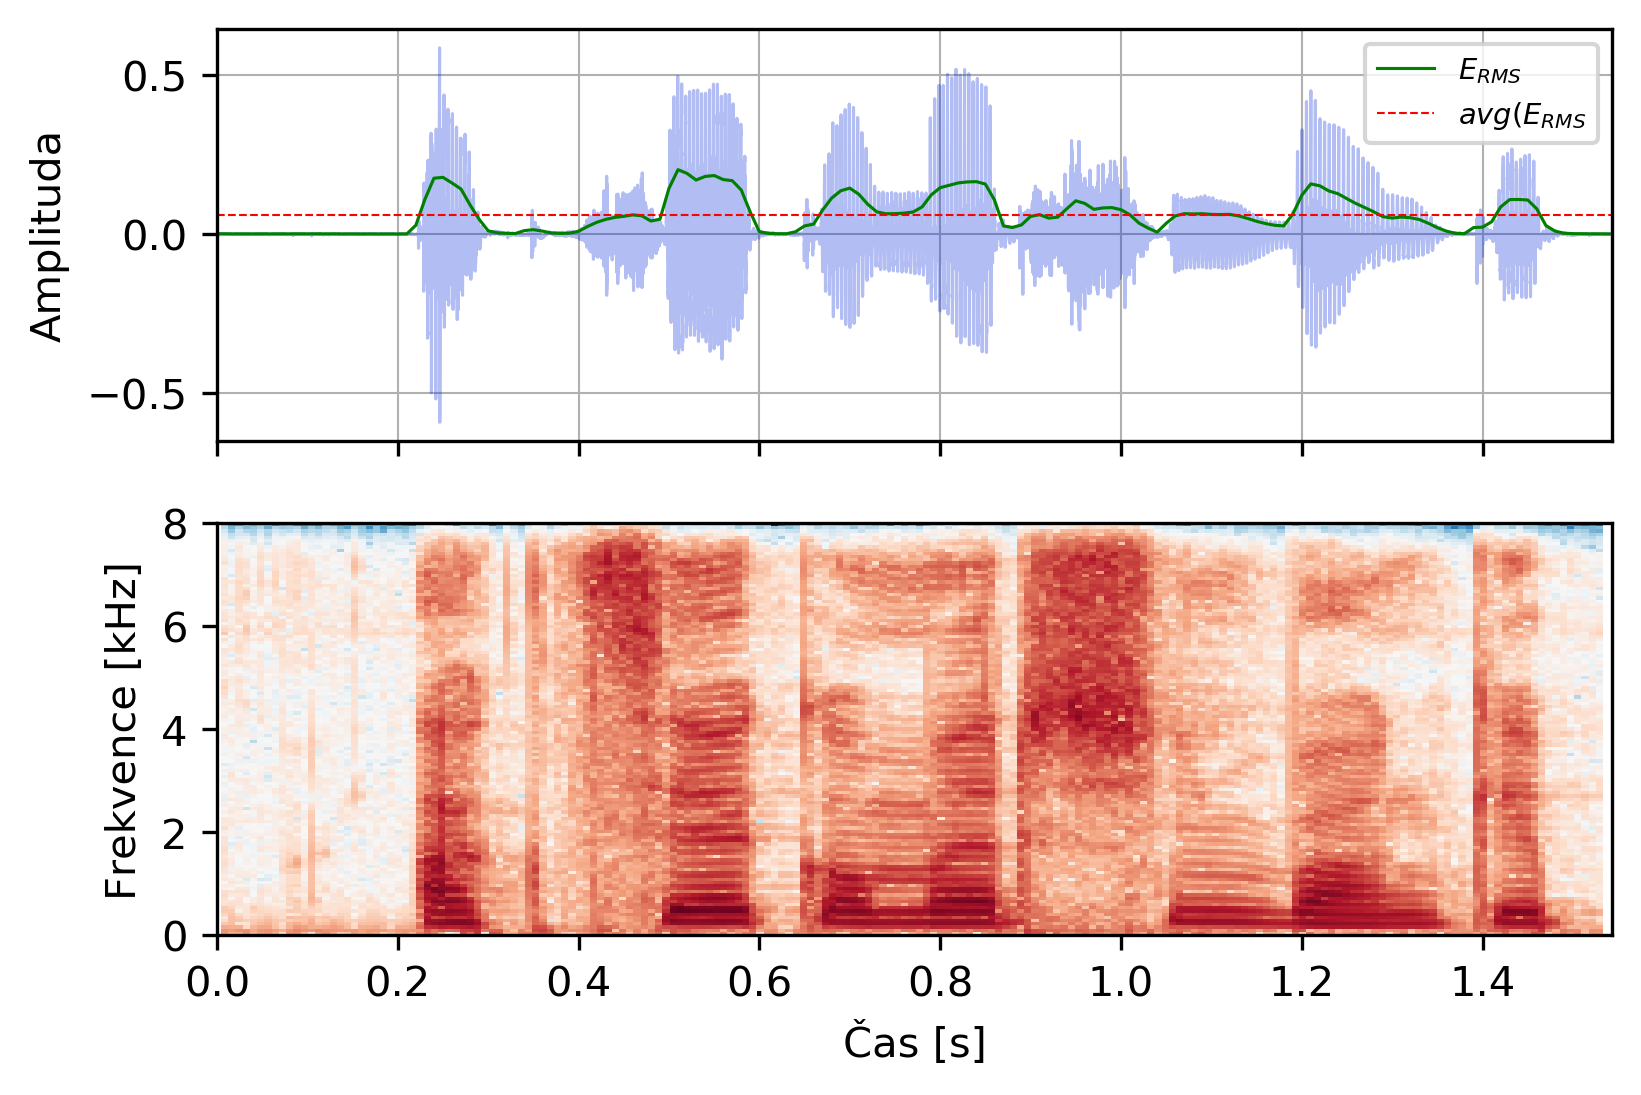
\includegraphics[width=\textwidth]{./ch5-construction/img/energy_spec_normal.png}
    \caption{Zdravý řečník}
    \label{fig:construction:analysis:comparison:normal}
  \end{subfigure}
  %
  \begin{subfigure}[b]{0.45\textwidth}
    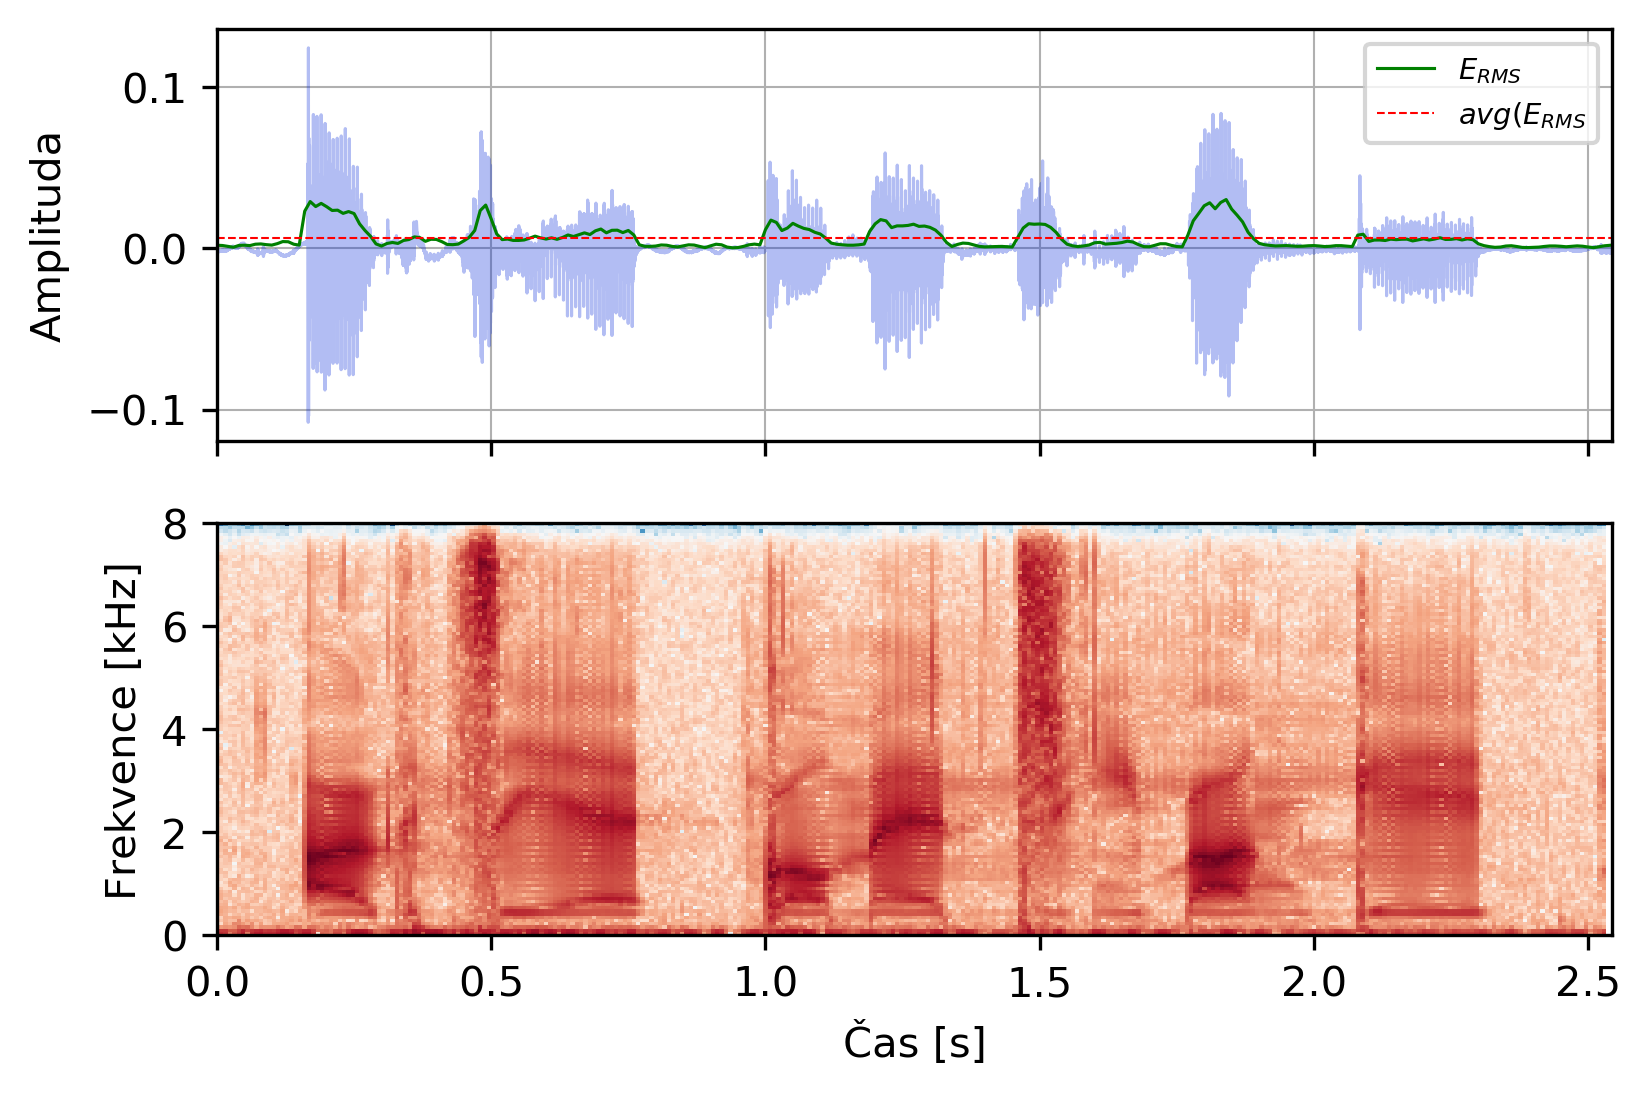
\includegraphics[width=\textwidth]{./ch5-construction/img/energy_spec_el.png}
    \caption{EL řečník}
    \label{fig:construction:analysis:comparison:el}
  \end{subfigure}
  \caption{Průběh a spektrogram promluvy a vyznačenou energií promluvy zdravého a EL řečníka.}
  \label{fig:construction:analysis:comparison}
\end{figure}

% \begin{figure}[hbpt]
%   \centering
%   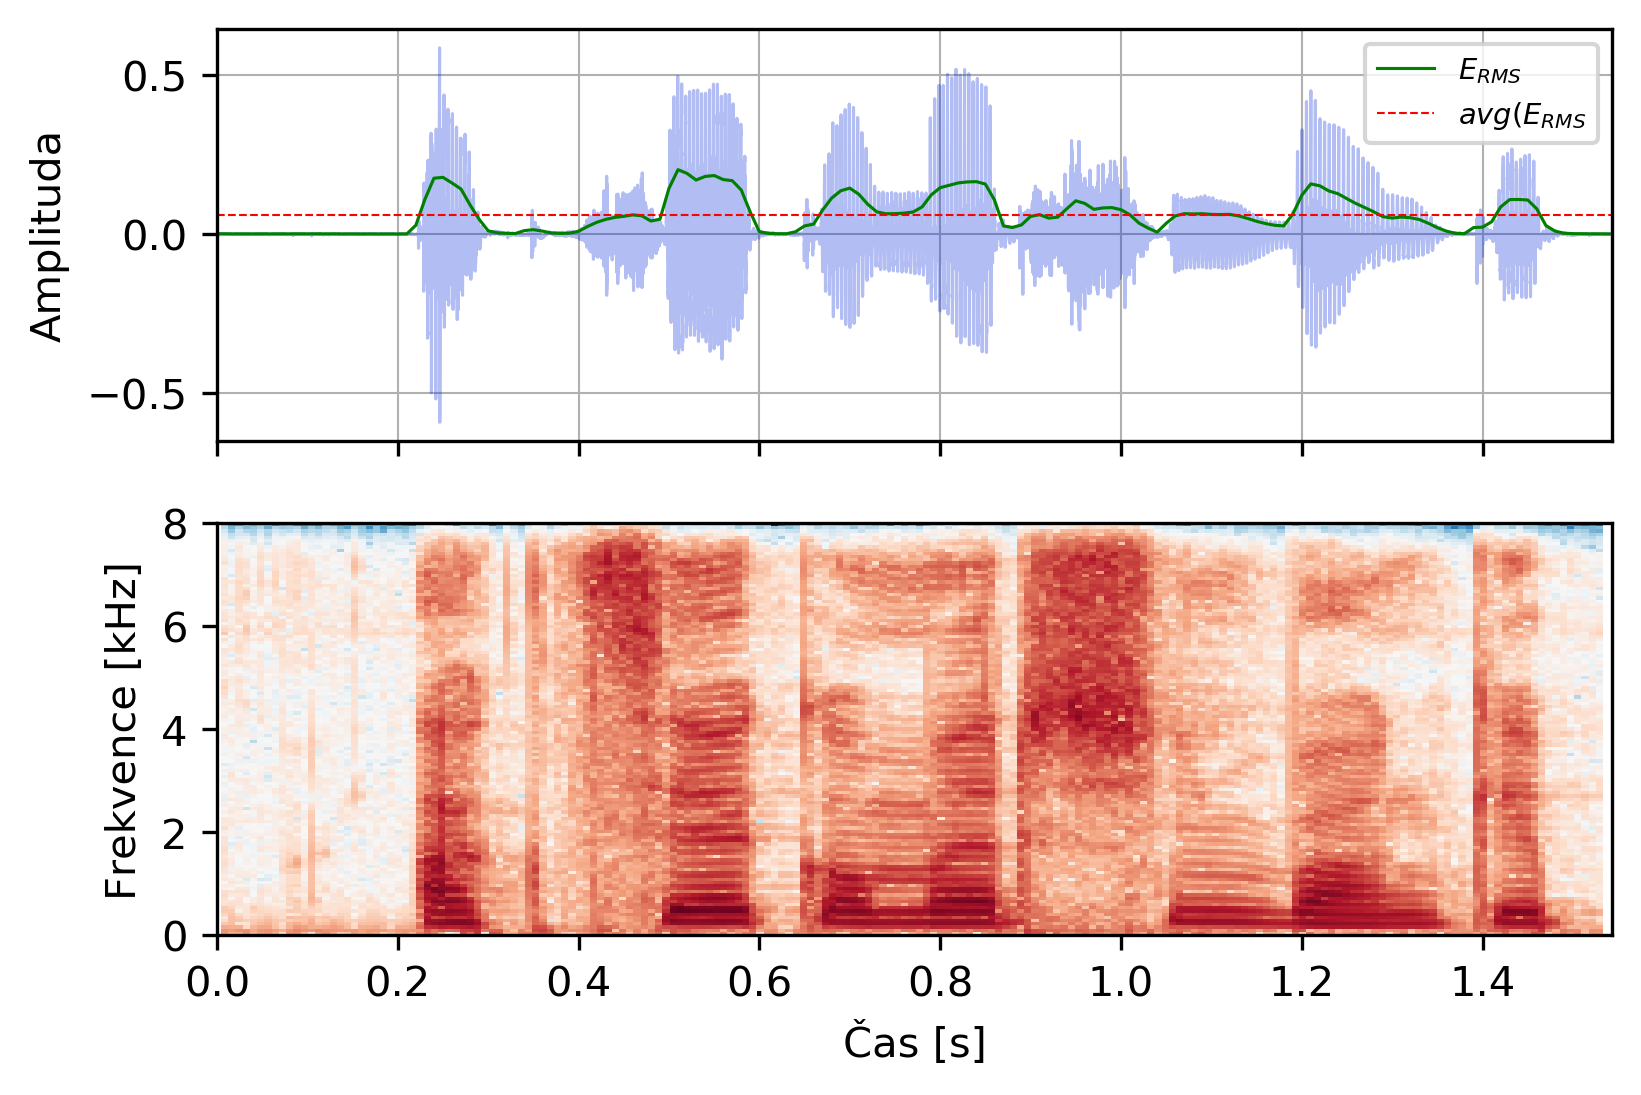
\includegraphics[width=0.9\textwidth]{./ch5-construction/img/energy_spec_normal.png}
%   \caption{Průběh a spektrogram promluvy a vyznačenou energií promluvy.}
%   \label{fig:construction:normal_speech}
% \end{figure}

Svou roli může hrát i snaha správně artikulovat. Při používání EL je to nezbytné, aby bylo produkované řeči alespoň trochu rozumnět. A pokud se dobře artikuluje, není snadné mluvit rychle. Při nahrávání bylo velmmi běžné, že v průběhu promluvy řečník udělal pauzu, aby mohl lépe umístit EL, protože jeho umístění má velký vliv na kvalitu produkované řeči. Nicméně je třeba říci, že tempo není a priory pro ASR systémy problém, protože různá délka fonémů je v relativně snadno modelována, viz část \ref{chap:asr:acoustic}.

Dalším způsobem jak ukázat rozdíly mezi promluvou zdravého a řečníka s EL, je srovnání ve frekvenční oblasti. Pro větší názornost jsou na obr. \ref{fig:construction:spectrogram} zobrazena společně spektra ukázkové promluva zdravého řečníka (\ref{fig:construction:spectrogram:normal}) a toho s EL (\ref{fig:construction:spectrogram:el}). Obsah obou promluv je identický a přesto jsou obě spektra odlišná.

Prvním markantním rozdílem je mnohem větší zastoupení šumu v úsecích \uv{ticha}, viz obr. \ref{fig:construction:spectrogram:el}. To je nepochyně způsobnemo samotným EL, který řečník nevypíná mezi jednotlivými slovy. Na obr. \ref{fig:construction:el_speech} je zřetelně patrný, zejména na průběhu energie, šum před prvním a druhým slovem promluvy. Zajímavá je přítomnost šumu v celém frekvenčním spektru, přestože EL produkuje konstantní buzení. To je ve spektru (obr. \ref{fig:construction:spectrogram:el}) viditelné jako výrazná souvislá linie v nízkých frekvencích. Přitomnost šumu ve vyšších frekvencích je způsobena umístěním mikrofonu, který je nalepen přímo na pokožku a tím pádem snímá namodulované vibrace, přenášené měkkou tkání. Tento fakt se potvrdil v dalších etapách nahrávání (viz část \ref{chap:realisation:corpus}), kde je použit studiový mikrofon vzdálený od úst minimálně 15 cm a tyto vibrace již nezaznamenává. Nicméně z pohledu použitelnosti nějakého budoucího systému je nezbytné počítat i se situací, kdy mikrofon zaznamenává i vibrace přenášené tkání.

Dalším významným rozdílem je absence vyšších frekvencí u většiny produkovaných fonémů. Vyjímku tvoří afrikáty $/c/$ a $/\check{c}/$, u kterých jsou hlasivky (u zdravého jedince) v klidu, a vznikají uvolněním nahromaděného vzduchu v dutině ústní\footnote{Nahromadění vzduchu je realizováno přitisknutím jazyka k přední/zadní části horního patra.} \cite{Psutka2006}. U těchto fonému není, u  řečníka po TL, mechanizmus produkce těchto fonémů ovlivněn. Problémem teoreticky může být zdroj vzduchu, jelikož jej z plic není možné dostat do dutiny ústní, ale jak už bylo zmíněno (a spektrogram to potvrzuje) zkušený uživatel EL se dokáže adaptovat.

Absence vyšších frekcencí se dá vysvětlit použitím EL, kde samotný EL má vždy konstantní frekvenci buzení a dále tím, že nedochází k modulaci ve všech dutinách vokálního traktu. Nicméně nejdůležitější složky, zajišťující srozumitelnost, se vyskytují ve frekvenčním pásmu od 1 kHz do 3 kHz. Vyšší frekvence se a priory podílejí na zabarvení hlasu.

\begin{figure}[htpb]
  \centering
  \begin{subfigure}[b]{0.4\textwidth}
    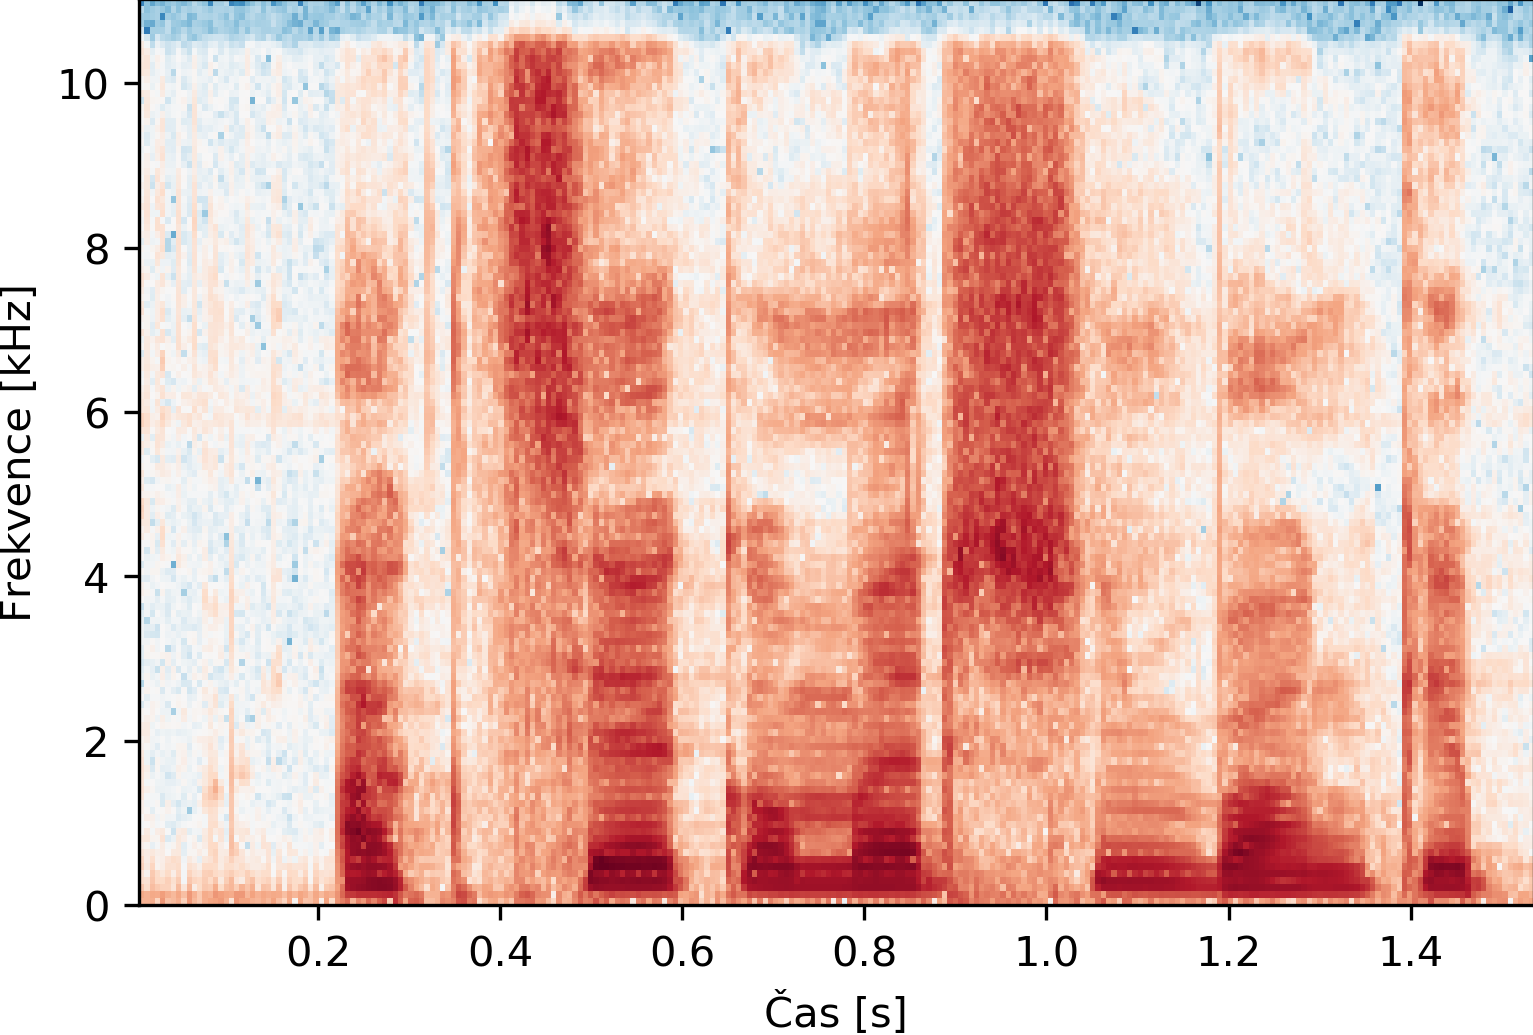
\includegraphics[width=\textwidth]{./ch5-construction/img/spectrogram_normal.png}
    \caption{Zdravý řečník}
    \label{fig:construction:spectrogram:normal}
  \end{subfigure}
  %
  \begin{subfigure}[b]{0.4\textwidth}
    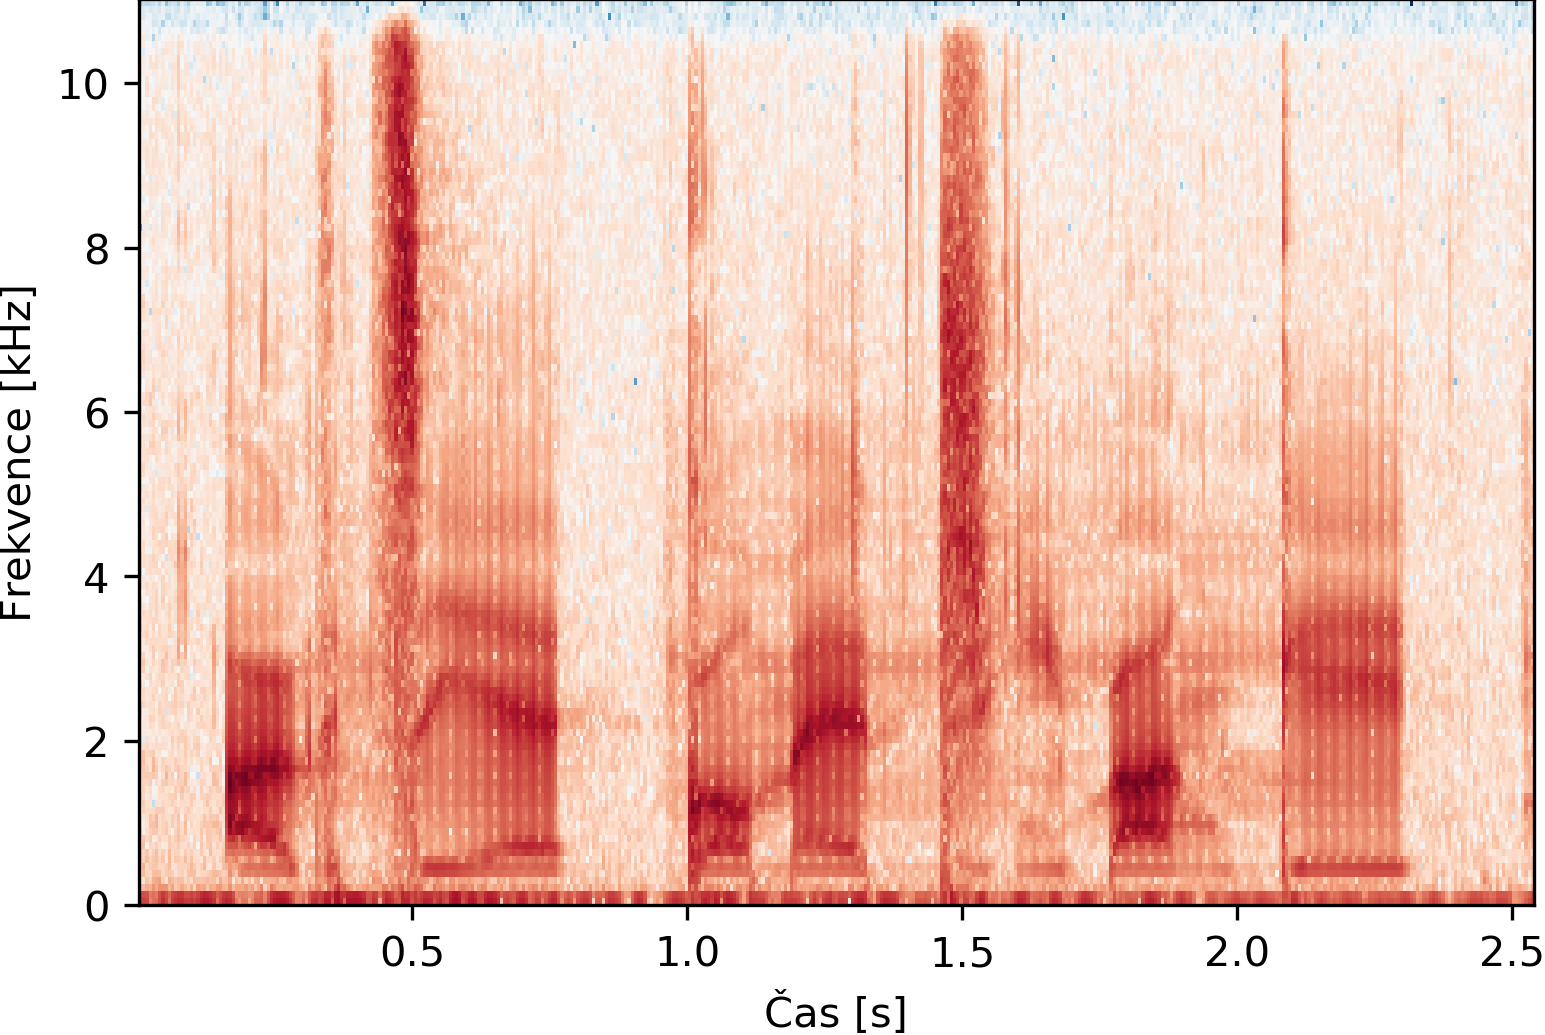
\includegraphics[width=\textwidth]{./ch5-construction/img/spectrogram_el.png}
    \caption{EL řečník}
    \label{fig:construction:spectrogram:el}
  \end{subfigure}
  \caption{Spektrogram promluvy \uv{Akcie Komerční banky} dvou řečníků.}
  \label{fig:construction:spectrogram}
\end{figure}

Dalším způsobem jak porovnat řeč zdravého a EL řečníka je pomocí analýzy jednotlivých fonémů. Na obr. \ref{fig:construction:phonemes:k}, \ref{fig:construction:phonemes:m} a \ref{fig:construction:phonemes:c} jsou zobrazeny průběhy amplitudy v čase\footnote{Hodnoty času odpovídají časům výskytu v původní promluvě.} pro fonémy $/k/$, $/m/$ a $/\check{c}/$. V případě $/k/$ a $/m/$ (obr. \ref{fig:construction:phonemes:k} a \ref{fig:construction:phonemes:m}) se jedná o okluzivy, kde v prvním případě jde o neznělou plozivu a v druhém o znělou plozivu. Tyto fonémy obecně vznikají uzavřením vydechovaného proudu vzduchu pomocí artikulačních orgánů, což se projeví jako krátká pauza (tzv. okluze). Po té následuje náhlé jednorázové uvolnění překážky a únik nahromaděného vzduchu, tzv. exploze \cite{Psutka2006}. Takto popsáno to samozřejmě funguje u zdravého jedince, ale u EL řečníka jde sice o stejný mechanizmus, ale s tím rozdílem, že vzduch nepochází z plic, ale z hltanu. Dalším rozdílem je samozřejmě absence hlasivek.

Foném $/k/$ je tedy zástupcem neznělých fonémů, ty se vyznačují tím, že do jejich produkce nevstupují hlasivky, které jsou v klidu. Zdrojem buzení je tedy šum, viz část \ref{chap:asr}. Pokud se podíváme na průběh amplitudy v čase u zdravého řečníka (obr. \ref{fig:construction:phonemes:k:normal}), tak zde není vidět žádný periodický signál. Hlasivky jsou tedy opravdu v klidu. Oproti tomu u EL řečníka (obr. \ref{fig:construction:phonemes:k:el}) je jasně patrné, že je zde přítomno aktivní buzení vytvořené EL. Ve frekvenční oblasti je zobrazeno tzv. amplitudové spektrum, které znázorňuje vývoj amplitudy signálu ve frekcenci. V případě zdravého řečníka odpovídá vývoj předpokladům, není zde žádná výrazná frekvence a také nedochází k výraznému útlumu. Přestože se v obou případech jedná o stejný foném, tak z časového i frekvečního průběhu je zřejmé, že parametry signálu se u obou řečníku diametrálně liší.

\begin{figure}[htpb]
  \centering
  \begin{subfigure}[b]{0.45\textwidth}
    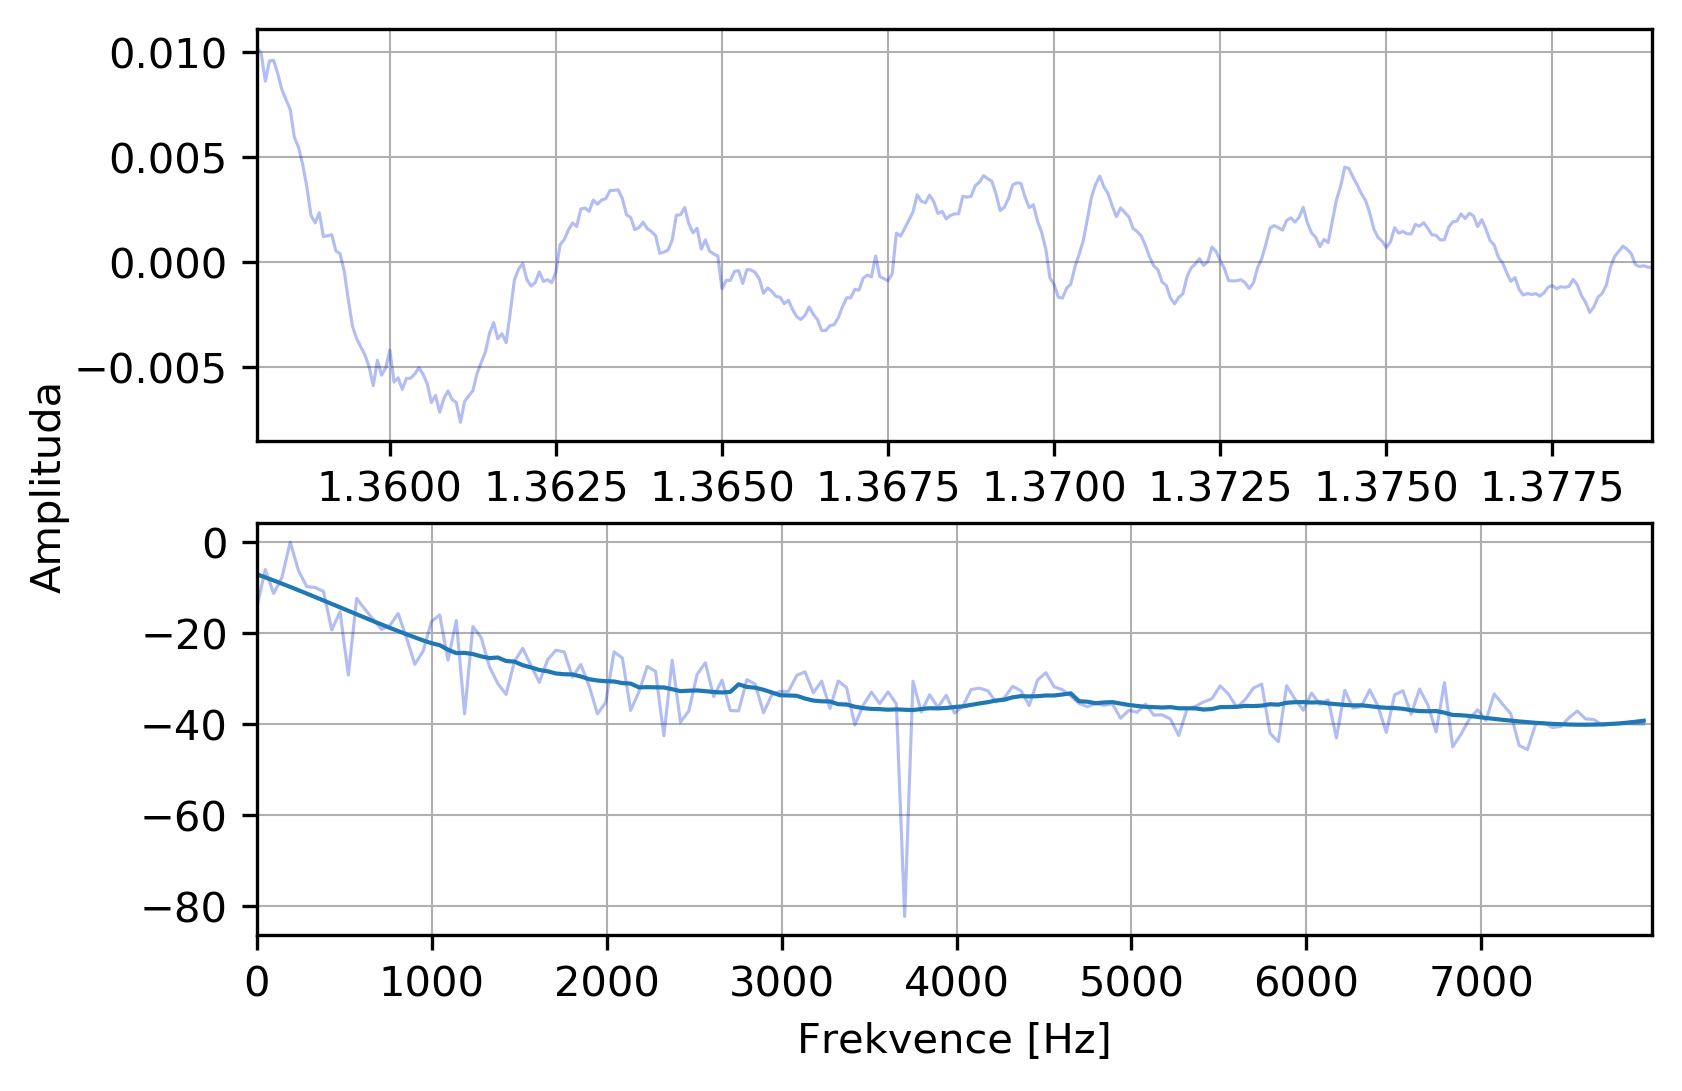
\includegraphics[width=\textwidth]{./ch5-construction/img/signal-normal_k.png}
    \caption{Zdravý řečník}
    \label{fig:construction:phonemes:k:normal}
  \end{subfigure}
  %
  \begin{subfigure}[b]{0.45\textwidth}
    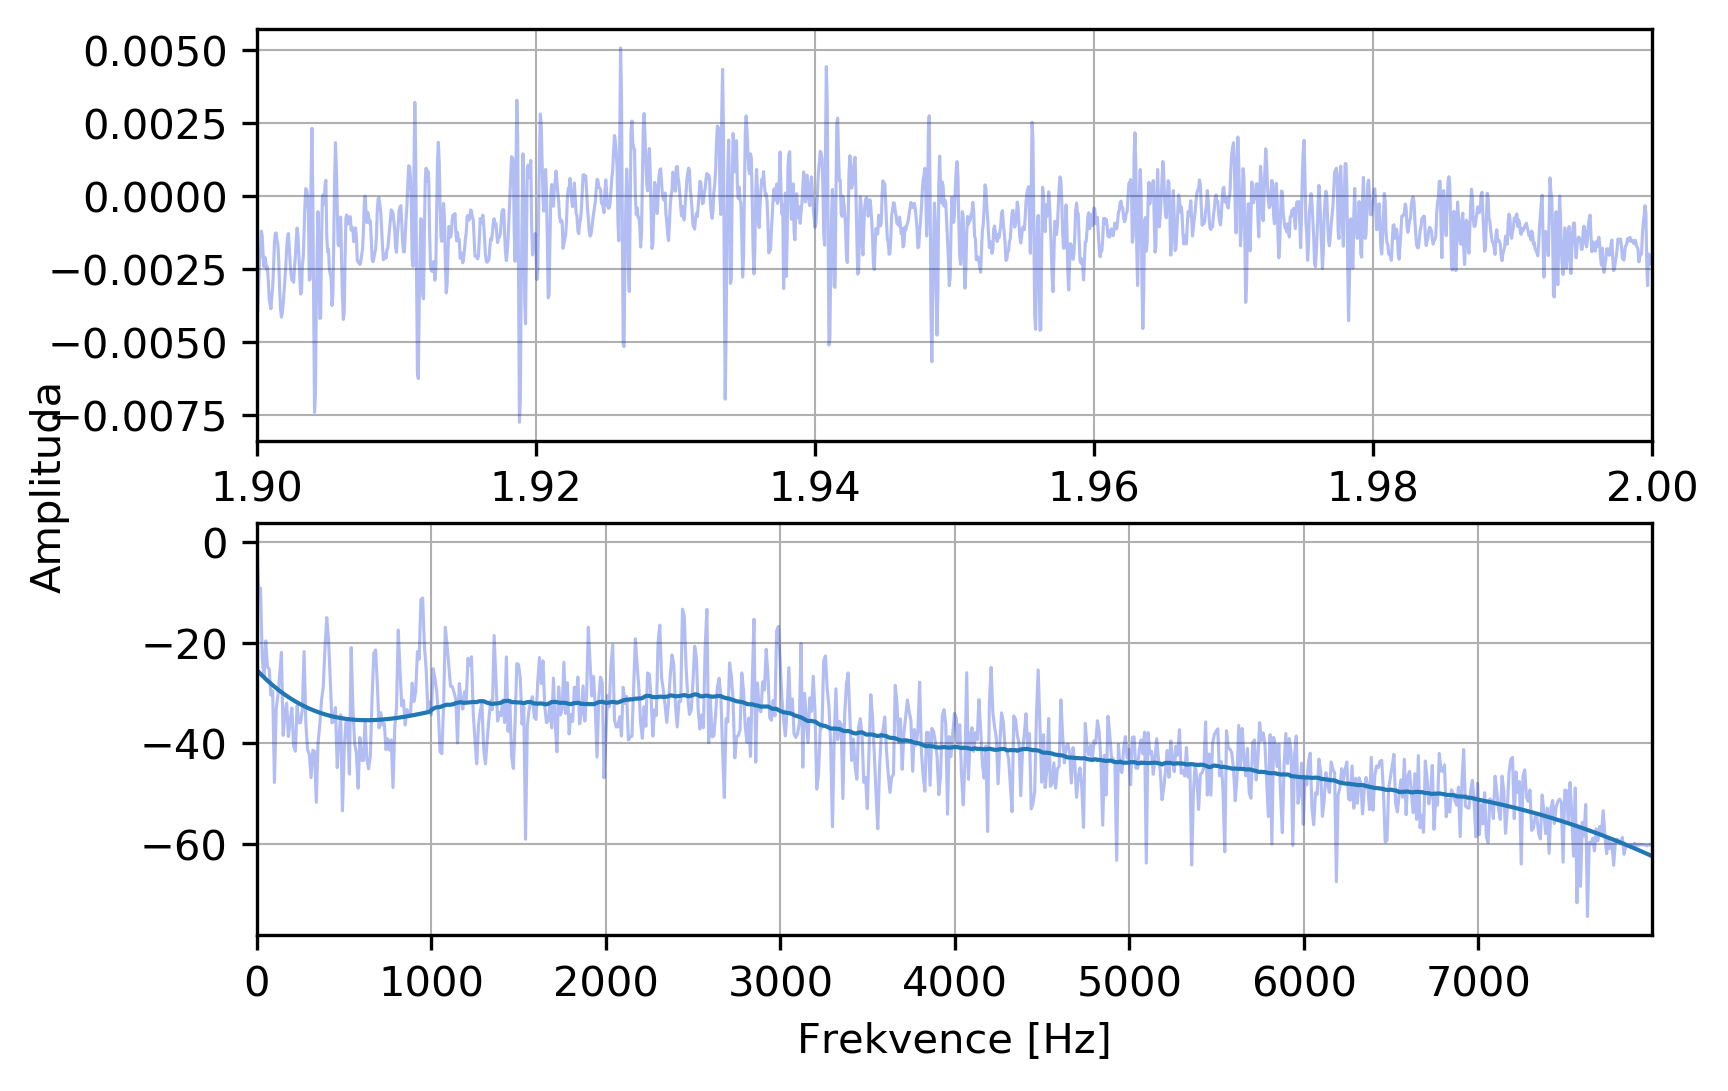
\includegraphics[width=\textwidth]{./ch5-construction/img/signal-el_k.png}
    \caption{EL řečník}
    \label{fig:construction:phonemes:k:el}
  \end{subfigure}
  \caption{Průběh amplitudy $/k/$ v časové a frekvenční oblasti fonému u normálního a EL řečníka}
  \label{fig:construction:phonemes:k}
\end{figure}

Jako druhý ukázkový foném slouží $/m/$. Jedná se o plozivu, ale v tomto případě znělou. U těchto fonémů hrají velký vliv hlasivky, protože jsou zdrojem buzení. Z obr. \ref{fig:construction:phonemes:m:normal} je toto buzení zřetelné ve formě perodického průběhu amplitudy. U EL řečníka (obr. \ref{fig:construction:phonemes:m:el}) je také vidět periodický signál, ale úplně jiného charakteru. Svým způsoběm dost podobný tomu, který je zřetelný u fonému $/k/$. Rozdíl je zřetelný i ve frekvenční oblasti, kdy u EL řečníka nedochází k útlumu ve střední oblasti frekvenčního spektra.

\begin{figure}[htpb]
  \centering
  \begin{subfigure}[b]{0.45\textwidth}
    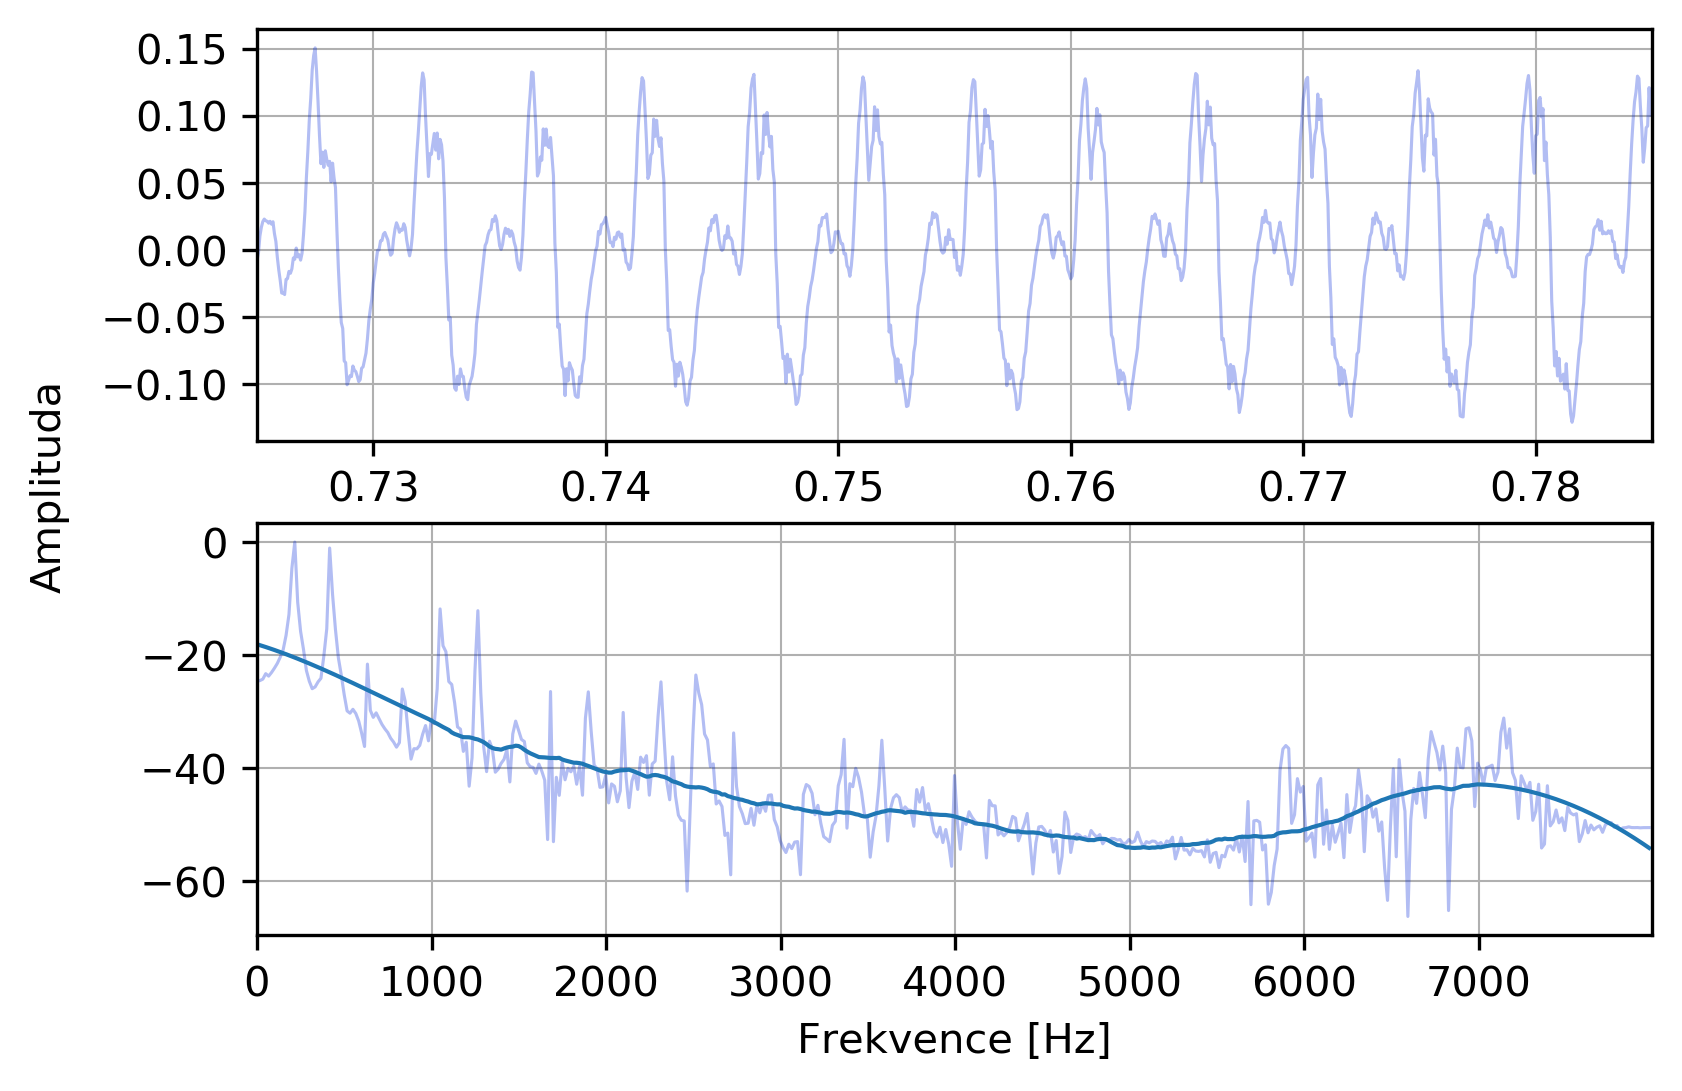
\includegraphics[width=\textwidth]{./ch5-construction/img/signal-normal_m.png}
    \caption{Zdravý řečník}
    \label{fig:construction:phonemes:m:normal}
  \end{subfigure}
  %
  \begin{subfigure}[b]{0.45\textwidth}
    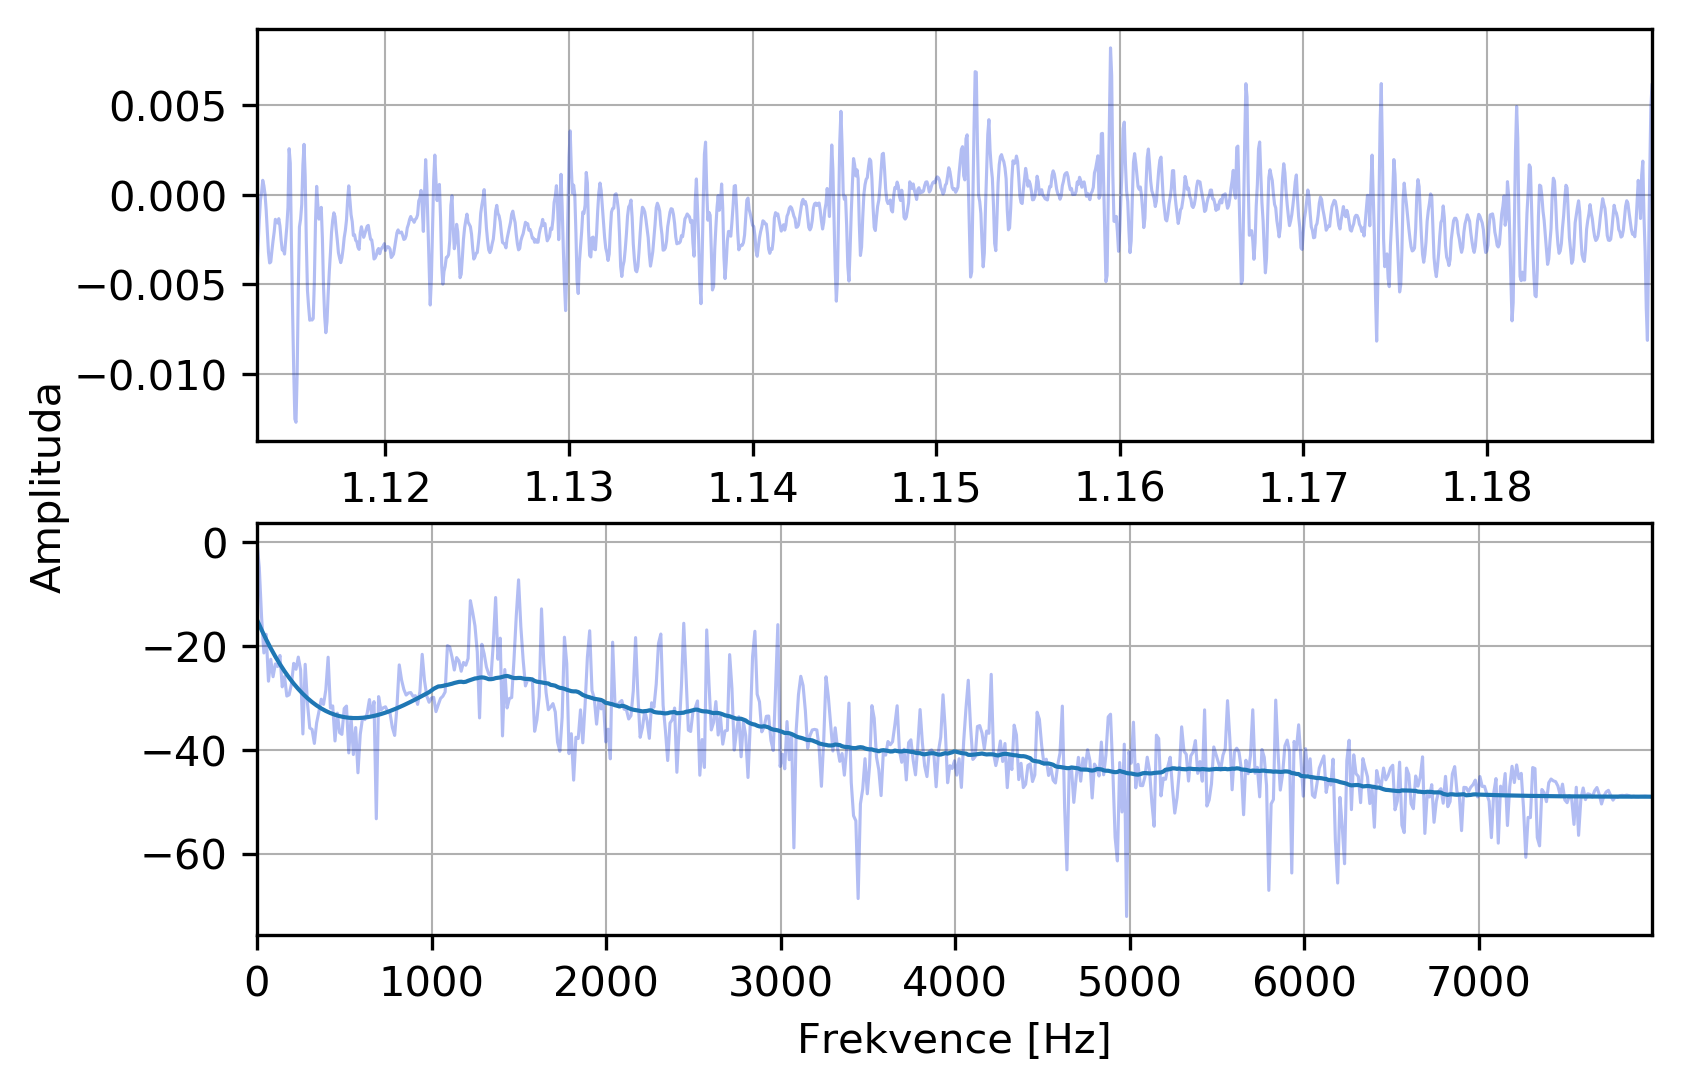
\includegraphics[width=\textwidth]{./ch5-construction/img/signal-el_m.png}
    \caption{EL řečník}
    \label{fig:construction:phonemes:m:el}
  \end{subfigure}
  \caption{Průběh amplitudy fonému $/m/$ v časové a frekvenční oblasti fonému u normálního a EL řečníka}
  \label{fig:construction:phonemes:m}
\end{figure}

Posledním úkázkovým fonémem je již zmiňované $/\check{c}/$. Jedná se o neznělý foném, který vzniká přiložením jazyku k zadní části horního patra. Tím je zadržen vzduch v dutině ústní a vzniká krátká pauza. Uvolněním pak dochází k explozi a vytvoření zvuku. \cite{Psutka2006} Do produkce se nezapojují hlasivky a produkovaný zvuk by měl být dostatečně intenzivní, aby jej (v případě EL řečníka) tolik neovlivňoval EL. Tím pádem by měl být průběh signálu, u obou řečníků podobný, a to jak v časové, tak i ve frekvenční oblasti, viz obr. \ref{fig:construction:phonemes:c}.

\begin{figure}[htpb]
  \centering
  \begin{subfigure}[b]{0.45\textwidth}
    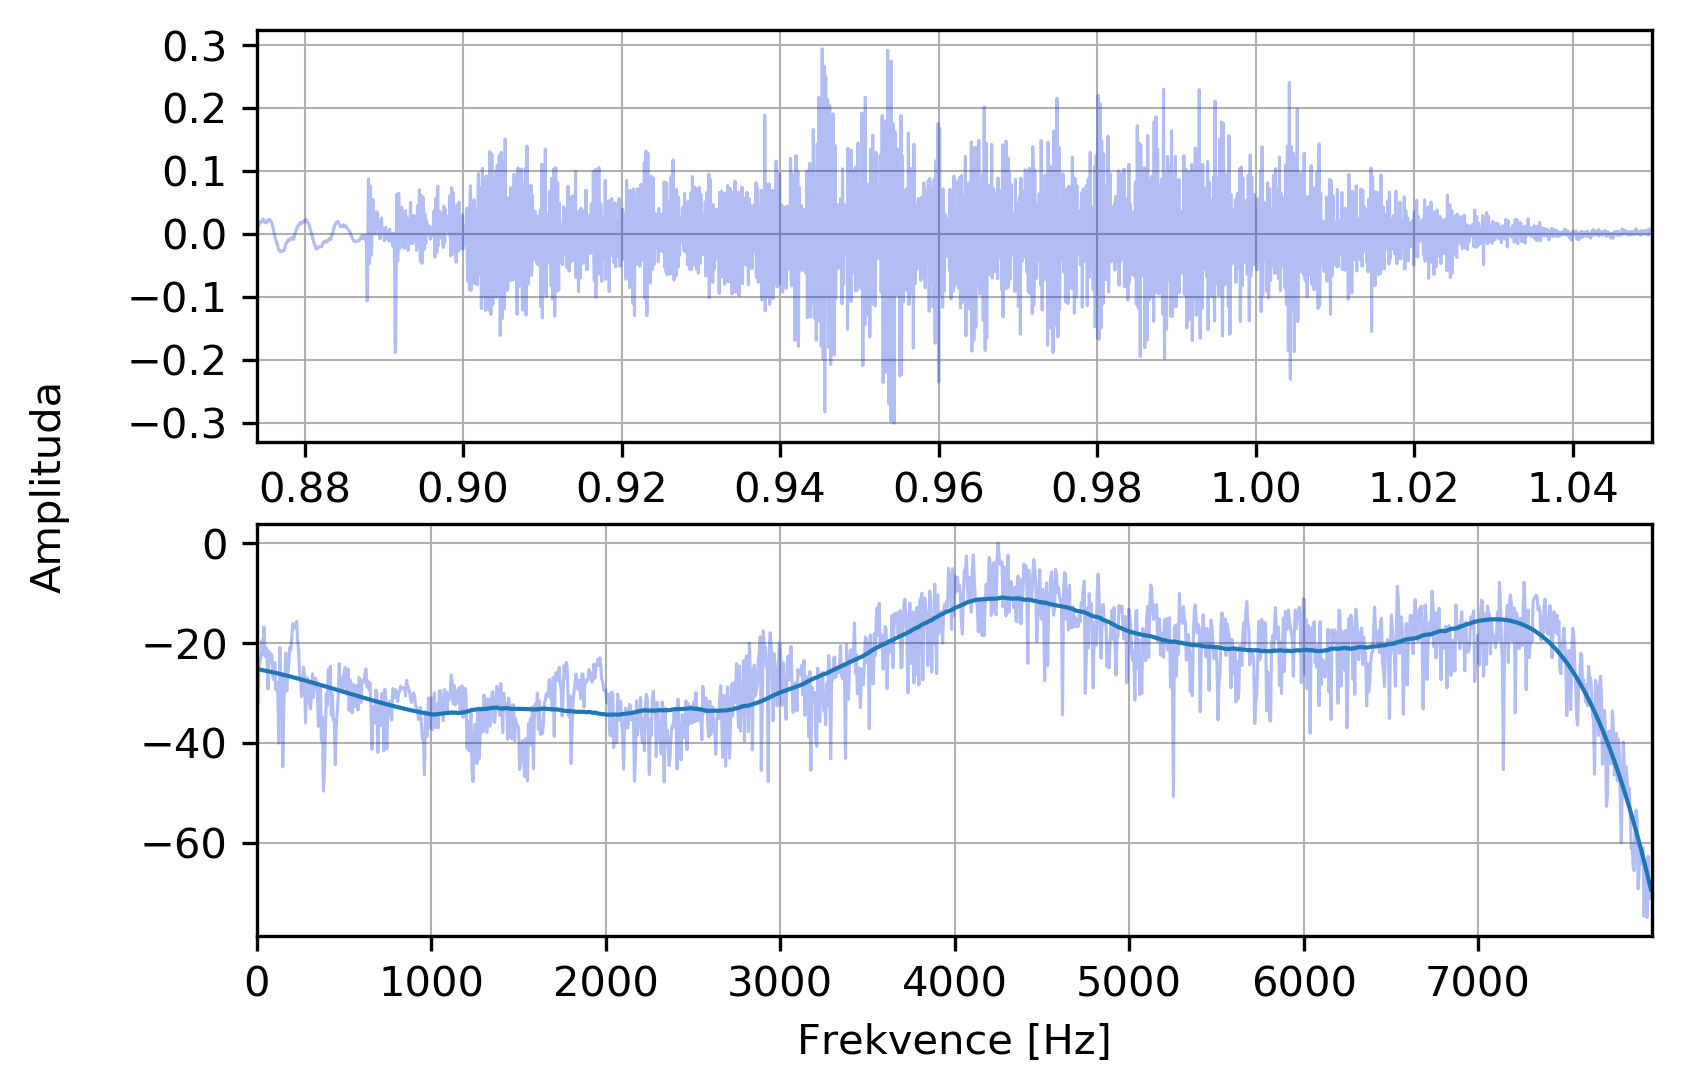
\includegraphics[width=\textwidth]{./ch5-construction/img/signal-normal_c.png}
    \caption{Zdravý řečník}
    \label{fig:construction:phonemes:c:normal}
  \end{subfigure}
  %
  \begin{subfigure}[b]{0.45\textwidth}
    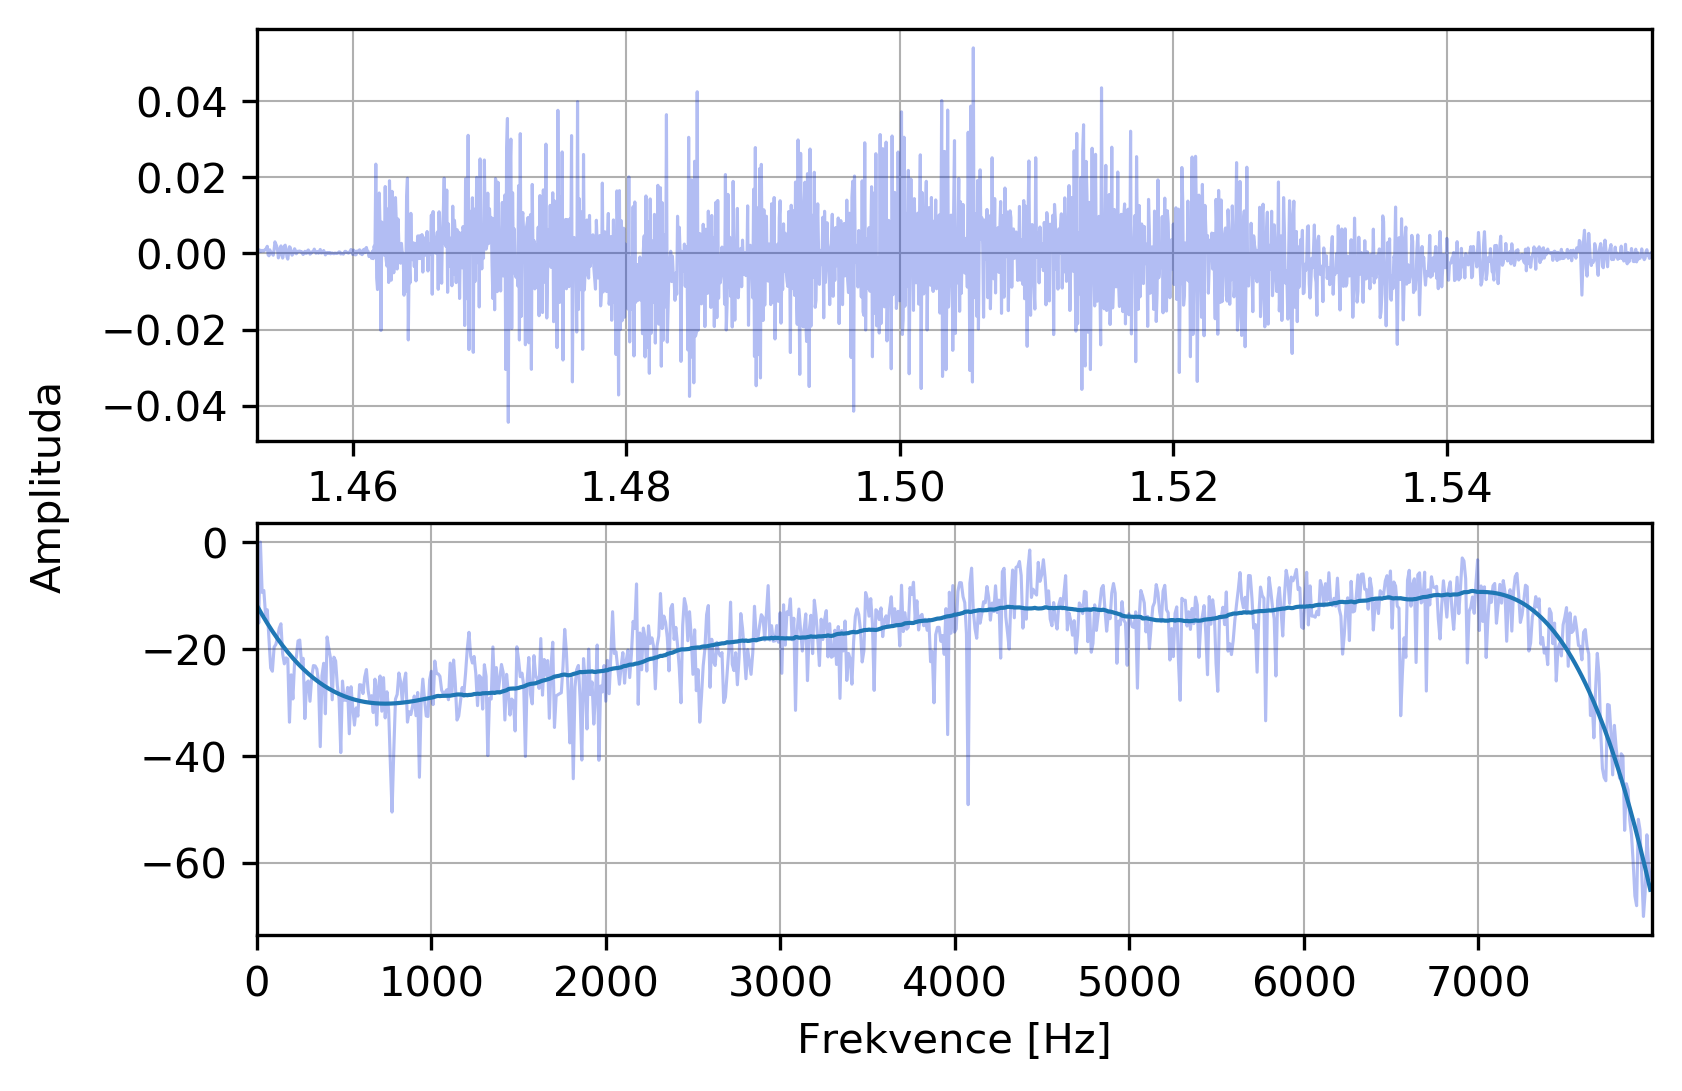
\includegraphics[width=\textwidth]{./ch5-construction/img/signal-el_c.png}
    \caption{EL řečník}
    \label{fig:construction:phonemes:c:el}
  \end{subfigure}
  \caption{Průběh amplitudy fonému $/\check{c}/$ v časové a frekvenční oblasti fonému u normálního a EL řečníka}
  \label{fig:construction:phonemes:c}
\end{figure}

Z doposud provedené analýzy plyne, že EL řeč je v mnoha charakteristikách odlišná od té produkované zdravým řečníkem. Zejména u porovnání ve frekvenční oblasti (obr. \ref{fig:construction:phonemes:k} a \ref{fig:construction:phonemes:m}) je to nejvíce patrné.
% Tento fakt nepochybně přispívá k tomu, že standardní obecné modely rozpoznávání řeči nedosahují takové přesnosti jako v případě bežné promluvy, viz dále.

% \csvautotabular{./ch5-construction/test.csv}

% !TEX root = ../thesis.tex
% \section{Akustický model}
% \label{chap:construction:am}

% \todo{Tady úplně nevim jak tahle sekce byla myšlená. Popsat akustický model u obecného modelu?}{TBD}

% Z provedené analýzy plyne, že pořízený EL korpus se svým obsahem odchyluje od standardního řečového korpusu používaného k trénování běžných akustických modelů. Otazkou je zda odlišné parametry EL řeči jsou natolik jiné, aby si s nimi obecný na řečníkovi nezávislý akustucký model s těmito rozdíly neporadil.

% Tento obecný akustický model je postaven na HMM-DNN modelu, konkrétněji TDNN síti, viz \ref{chap:asr:acoustic:DNN}. K natrénování pousloužil řečový korpus obsahující \textbf{TBD}...

% K ověření schopností ASR systému ...

% !TEX root = ../thesis.tex
% \section{Jazykový model}
% \label{chap:construction:lm}

% TBD

% Popsat trifónový jazykový model s 1M slov co byl použit k otestování na obecném modelu?

% Popsat fonémový zerogramový jazykový model?

% !TEX root = ../thesis.tex
\section{Aplikace obecného systému rozpoznávání a dosažené výsledky}
\label{chap:construction:results}

Z provedené anylýzy plyne, že získaný EL korpus je odlišný od \uv{standardního} řečového korpusu, který se běžně používá k trénování obecných akustických modelů. Tyto modely jsou nezávislé na řečníkovi a vyznačují se robustnostní. Je tedy otázka, zda takovýto model nebude schopen pracovat s EL daty.

K ověření byl vytvořen TDNN akustický model (více o těchto modelech v části \ref{chap:asr:acoustic:DNN}), který byl natrénován daty z korpusu čítající $1000$ hodin promluv od velkého počtu řečníků. Celkový počet HMM stavů je \textbf{XXXX}.

Jazykový model je postaven na trigramech a k jeho natrénování posloužil textový korpus čítající velké množství novinových článků, webových reportáží, fílmových titulků a dalších textových záznamů. Slovník jazykového modelu čítá více než $1$ milion unikátních slov.

Testovacím vstupem vytvořeného ASR systému jsou data z EL korpusu. Celková slovní přesnost, počítaná podle vzorce (\ref{eq:asr:decoding:acc}), dosáhla hodnoty $18,49\ \%$\footnote{Dosaženo na state-of-the-art ASR systému v době psaní práce. V době vytvoření EL korpusu (kolem roku 2011) převládaly HMM-GMM akustické modely. Tento systém dosáhl přesnosti na slovech $12,59\ \%$.}.

Dosažený výsledek zřetelně ilustruje odlišnost EL domény, protože obecný na řečníkovi nezávislý systém s velkým jazykovým modelem není schopen obstojně rozpoznat EL promluvu.

Pokud jsou k natrénování akustického modelu (taktéž využívajícího TDNN síť) použita pouze data\footnote{Korpus byl náhodně rozdělen na trénovací a testovací sadu v poměru $90\ \%$ trénovací a $10\ \%$ testovací sada. Toto rozděleni je použito ve všech experimentech.} z EL korpusu, tak výsledná slovní přesnost dosáhla hodnoty $83,33\ \%$, opět počítáno podle vzorce (\ref{eq:asr:decoding:acc}). Jazykový model je identický jako v případě obecného systému. Dosažený výsledek demostruje výhodu vytvoření individuálního modelu z EL nahrávek. Zároveň ukazuje schopnost akustického modelu namodelovat specifika EL řeči. Přestože je výsledek individuálního modelu výrazně lepší, než obecného modelu zpracovájící EL promluvy, tak zdaleka nedosahuje hodnot nejlepších ASR systémů, které jsou schopny v ideálních podmínkách dosahovat více než $90\ \%$ slovní přesnosti.


%Z dosaženého výsledku je patrné, že EL doména je diametrálně odlišná od bežné řeči, pro které jsou ASR systémy vytvářeny. Navíc, pokud se vezme v potaz náročnost získání potřebných dat pro natrénování obecného modelu, tak se jako jediná schůdná varianta jeví vytváření individuálních modelů pro každého řečníka. To znamená, že model je trénovaný pouze z dat odpovídající konkreténímu řečníkovi a často i účelu použití. K vytvoření takového modelu je zapotřebí řádově méně dat, při dosažení podobného výkonu. Stinnou stránkou je případná menší robustnost modelu. Čistě logicky tento model bude fungovat pouze s konkrétním řečníkem a ještě jen v situacích, které odpovídají trénovacím datům. U řečníků s EL může navíc hrát velký vliv samotný EL. Již při nahrávání se ukázalo, že jeho pozice může nepříznivě ovlivnit kvalitu řeči. Tento problém by však neměl významně ovlivňovat kvalitu modelu, protože tento fenomém je obsažen v datech.

\subsection{Hledání optimálních parametrů baseline modelu}
\label{chap:construction:results:baseline}

%Co se však ukázalo jako potencionálně problematické, je stabilita parametrů produkované řeči v dlouhodobém časovém úseku. Více o tomto problému pak v části \ref{chap:construction:normalization:quality}. K zodpovězení nejdůležitější otázky, jestli takový model vůbec může fungovat, stačí získaná data z první etapy nahrávání a ta obsahují řeč s relativně konzistentními parametry.

V rámci ověřování funkčnosti individuálního modelu je vhodné zkusit různé varianty k nalezení optimálních parametrů modelu. Hlavními uvažovanými hyperparametry jsou vzorkovací frekvence audio nahrávek a počet \textit{HMM} stavů. Originální pořízené nahrávky mají vzorkovací frekvenci rovnu $44,1\ kHz$, pro úlohu rozpoznávání EL řeči je to však zbytečně vysoká frekvence, protože nejhodnotnější informace je obsažena u EL řeči ve frekvenčním pásmu do $4\ kHz$. Vyšší frekcence a priory ovlivňují zabarvení hlasu a další individuální charakteristiky. \cite{Psutka2006} Samotná EL řeč však obsahuje věci, které běžná řeč neobsahuje a tak je otázka, zde vhodnější vzorkovací frekvence rovna $8\ kHz$ nebo lépe $16\ kHz$.

Počet stavů modelu ovliňuje množsví modelovaných trifónů, viz \ref{chap:asr:acoustic:HMM}. Čím více akustických jednotek je modelováno, tím více musí mít HMM model unikátních stavů. Stinnou stránkou je, že čím více stavů model má, tím více trénovacích dat je potřeba k natrénování robustního modelu. Celkem jsou uvažovány modely s $1024,\ 2048$ a $4096$ stavy.

%Jen pro vysvětlení je dobré zmínit, že \textit{HMM} stav představuje model jedné uvažované akustické jednotky (nebo skupiny jednotek s podobnými parametry). Počet stavů nám tedy říká, kolik takových jednotek model dokáže rozlišit. Čím více stavů, tím více jednotek (menších skupin) je modelováno. Teoreticky tak model s více stavy je lepší. Nicméně k natrénování jednotky je potřeba určité množství dat a tím pádem je pro model s vyšším počtem stavů logicky potřeba větší množství trénovacích dat. Samozřejmě fonetická sada neobsahuje $4096$ fonémů, neobsahuje ani $1024$ fonémů\footnote{Ve skutečnosti obsahuje 42 českých fonémů.}. U těchto modelů se pak používá nějaký druh \textit{n-gramové} reprezentace fonémů, nejčastěji pak trifóny.

Takže při uvažování vzorkovacích frekvencí $8\ kHz$ a $16\ kHz$ bylo natrénováno $6$ modelů. K vytvoření akustických modelů je použit HTK-Toolkitu v3.4., který je určen k vytváření \textit{HMM} modelů. Při trénování je nejprve vytvořen monofónový akustický model s jedním gaussiánem pro každý stav. Ten poté slouží jako základ pro trifónové modely. Výsledný trifónový model využívá směs gaussiánů tak, jak je to popsáno v \ref{chap:asr:acoustic:GMM}. Celý proces trénování je znázorněn na obr. \ref{fig:construction:results:baseline:hmm:training}.

\begin{figure}[hbpt]
  \centering
  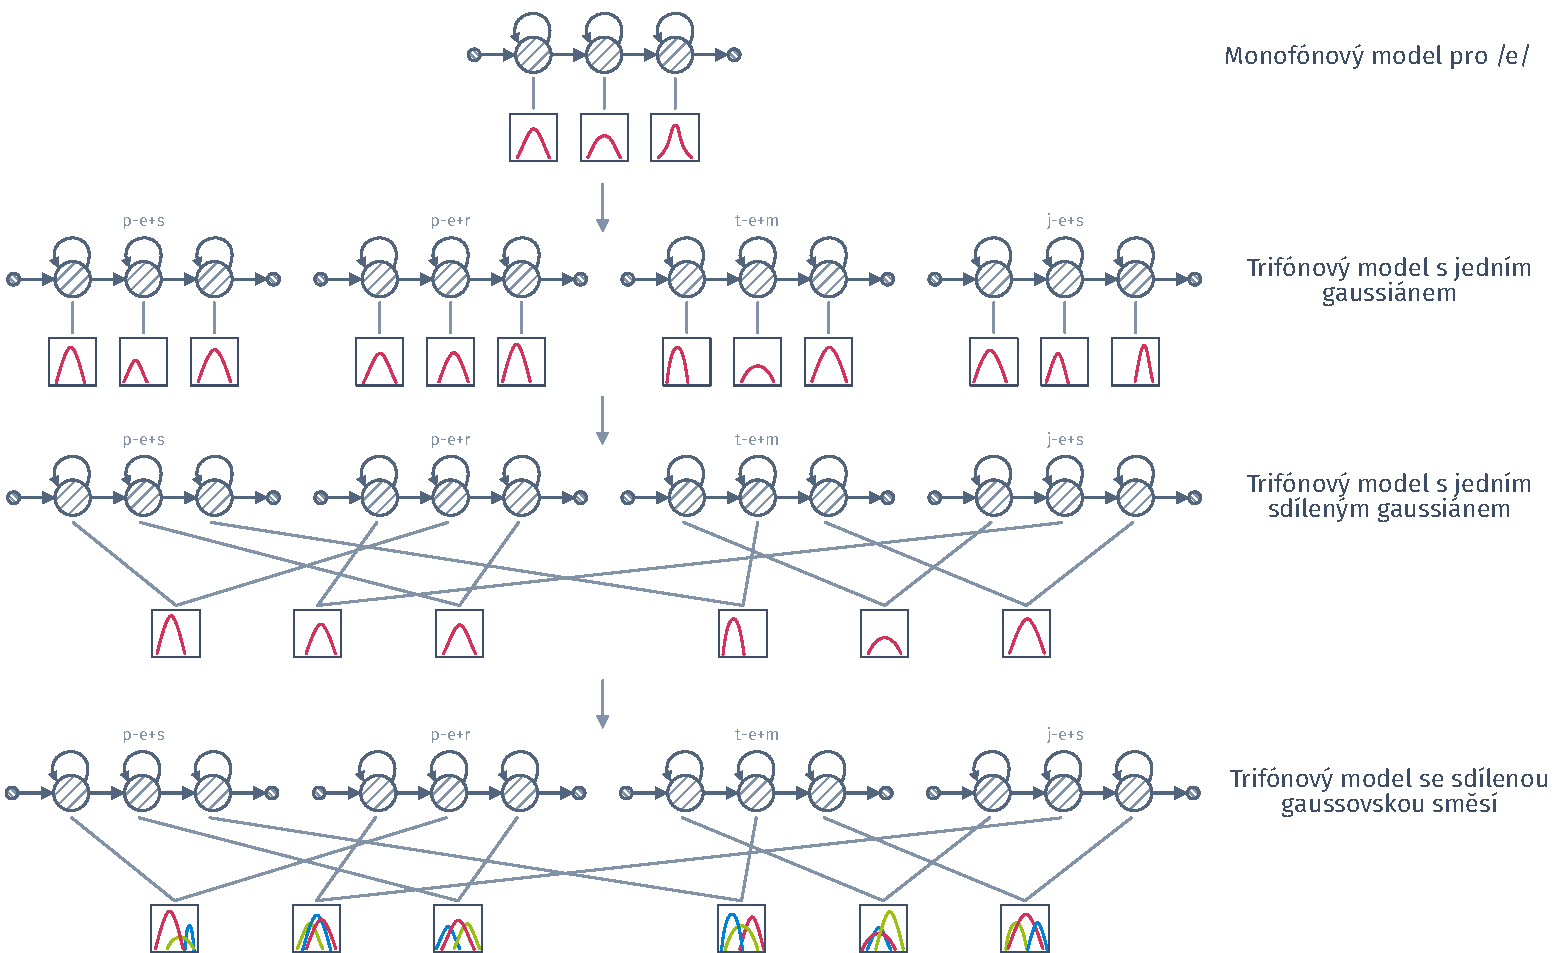
\includegraphics[width=0.9\textwidth]{./ch5-construction/img/hmm-training.pdf}
  \caption{Princip trénování HMM-GMM modelu}
  \label{fig:construction:results:baseline:hmm:training}
\end{figure}

Snahou je nalezení vhodných parametrů baseline modelu, zejména pak toho akustického. K tomu je potřeba minimalizovat vliv jazykového modelu. Z tohoto důvodu je použit speciální zerogramový jazykový model. Standarně, když se mluví o jazykovém modelu, se předpokládá, že základní jednotkou modelu je slovo. Pro ně jsou počítány četnosti z trénovacích dat a vytvořen model, viz část \ref{chap:asr:language}. Obecně, ale není nutné, aby základní jednotkou byla slova. V tomto případě je mnohem lepší vytvořit model jehož základní jednotkou je foném, protože ten je výstupem akustického modelu. Výstupem ASR systému tak bude sekvence fonémů, která z praktického pohledu není úplně užitečná, ale pro testování vlastností akustického modelu se hodí dokonale. V rámci této práce je takovýto model nazýván jako fonémový zerogramový jazykový model. Velikost slovníku tohoto modelu odpovídá velikosti fonémové sady a tady pravděpodobnost libovolného fonému je rovna $P(w_n) = 1/N$\footnote{Označení $w_n$ může evokovat použití slov u jazykového modelu. Změna písmena by však mohla vést ke zmatení čtenáře, protože by byla použita nestandardní notace. Z tohoto důvodu je i pro speciální model použito označení fonémů $w_n$.}, kde $N=40$. Výsledná přesnost je tedy a priory závislá pouze na akustickém modelu. Akustická data byla parametrizována pomocí MFCC s 26 filtry, 12 kepstrálními koeficienty a energií. Příznakový vektor obsahuje první i druhou derivaci těchto koeficientů. Více o parametrizaci založené na procesu slyšení v části \ref{chap:asr:parametrization:hearing}.


% Funkce ASR systému lze popsat rovnící

% \begin{equation}
%   \argmax_W p\left(W | O\right) = \argmax_W p\left(O | W\right) p\left(W\right),
% \end{equation}

%\noindent kde $O$ reprezentuje sekvenci akustických příznaků a $W$ výstupní sekvenci znaků\footnote{Znakem tu může být myšleno písmeno, případně slovo.}. $P\left(O | W\right)$ je pravděpodobnost generování korektní pozorované sekvence, tedy korektní k akustickému modelu ASR systému. Pravděpodobnost $P\left(W\right)$ je a priorní pravděpodobnost konkrétní sekvence znaků $W$, jinými slovy jazykový model. K získání výsledků je tedy potřeba mít i tento model.

%Ten však není níjak ovlivněn řečníkem (pouze doménou použití systému) a není jej třeba upravovat pro potřeby řečníka s EL. Cílem experimentu je ověření funkčnosti ASR a nalezení optimálních parametrů akustického modelu. Z tohoto důvodu je potřeba co nejvíce eliminovat vliv jazykového modelu na celkovém výkonu ASR systému. Jak bylo zmíněno, funkcí $p\left(W\right)$ je určení nejpravděpodobnější sekvnce znaků. Pravděpodobnostní rozložení je získáno z velkého množství trénovacích textů. Toto natrénované rozložení by však velmi ovlivnilo výsledky experimentů, a proto je použít zerogramový monofónový model. Ten se vyznačuje tím, že všechny prvky slovníku mají stejnou pravděpodobnost rovnu $P(w_n) = \frac{1}{N}$, kde $N$ je počet položek ve slovníku. Monofónový model je navíc zvolen z toho důbodu, že fonetická sada je známa a obsahuje malý počet jednotek. Z pohledu jazykového modelu má libovolný výstup z akustického modelu stejnou pravděpodobnost výskytu a tím pádem se jazykový model nijak nepřispívá k celkové kvalitě ASR systému.

Tab. \ref{tab:construction:experiment:gmm} znázorňuje dosažené výsledky HMM-GMM modelů. Opět se potvrdilo, že individuální ASR systém s EL daty může fungovat. Pokud dosažené výsledky porovnáme s výsledky obecného modelu ($Acc_{word} = 18,49\ \%)$, tak i zde je vidět rapidní nárůst přesnosti ($78,63\ \%$ u nejhoršího individuálního GMM modelu). Ze získaných výsledků je zřejmé, že použití vzorkovací frekvence $16\ kHz$ je vhodnější. Oproti $8\ kHz$ je dosaženo zlepšení přesnosti o $1,41\ \%$ absolutně, tedy téměř $7\ \%$ relativně. Dodatečné experimenty ukázaly, že použití vyšší vzorkovací frekvence než $16\ kHz$ přinese jen zanedbatelné zlepšení.

Dálse se ukázalo, že počet stavů nehraje tak zásádní roli při posuzování kvality akustického modelu, jako vzorkovací frekvence. Z testované množiny počtu stavů dosáhl nejlepšího výsledku model, který měl maximálně $4096$ stavů, nicméně oproti modelu s $1024$ stavy je nárůst přesnosti pouze $0,4\ \%$ absolutně v případě $16\ kHz$ modelů, což není tak významné. Logicky se nabízí otázka, proč nezkusit ještě více stavů? Odpověď se skrývá ve skutečném počtu stavů modelu s maximálním počtem $4096$ stavů. Slovíčko \uv{maximálním} je zde podstatné. Algoritmus trénování akustického modelu se snaží rozdistribuovat všechny možné akustické jednotky (v tomto případě trifóny) do maximálního počtu stavů. Pokud chceme méně stavů než jednotek, tak dochází k určité formě shlukování (za pomocí fonetického rozhodovacího stromu) \cite{Holmes2001}. Pokud je dostatek dat k natrénování konkrétního shluku, je tento shluk akceptován, pokud není dostatečné množství, je tento shluk spojen s jiným, který je svými parametry nejblíže. V případě, že je k dizpozici dostatek dat k natrénování maximálního počtu stavů má model tento počet stavů. Pokud není dostatek dat, může mít model méně stavů. U modelu s maximálním počtem $4096$ stavů je skutečný počet stavů $3257$, tzn. i kdyby se trénoval model s $8192$ stavy, tak by se tato hodnota změnila jen velmi málo.

%Pro doplnění, fónémový akustický model dosáhl přesnosti $54,49\ \%$ pro $8\ kHz$ a $62,30\ \%$ pro $16\ kHz$.

\begin{table}[htpb]
  \centering
  \def\arraystretch{1.5}
  \pgfplotstabletypeset[
    col sep=semicolon,
    string type,
    columns/model/.style={column name={Počet HMM stavů}, column type={c}},
    columns/8k/.style={column name={8 kHz}, column type={r}},
    columns/16k/.style={column name={16 kHz}, column type={r}},
    every head row/.style={
      before row={
        \toprule & \multicolumn{2}{c}{$Acc_{p}\ [\%]$} \\
      },
      after row={
        \cmidrule(r){1-1}
        \cmidrule(l){2-3}
      }
    },
    every last row/.style={after row={\bottomrule}},
  ]{./ch5-construction/tabs/01-frequency.csv}
  \caption{Vliv frekvence na kvalitu modelu.}
  \label{tab:construction:experiment:gmm}
\end{table}

Hledání optimálních parametrů baseline modelu bylo realizováno na přelomu let $2013$ a $2014$. V tuto dobu byly stále dominantní GMM modely. Z tohoto důvodu byl později tento experiment zopakován s HMM-DNN akustickým modelem. Vstupem modelu byla stejná MFCC parametrizace s 26 filtry, 12 kepstrálními koeficienty plus energie, delta a delta-delta příznaky. Tato parametrizace je provedena na mikrosegmentu $t$ a jeho okolí $t-5$ a $t+5$. Každý mikrosegment má délku $10\ ms$. Samotná síť se skládá z 6 vrstev, každá s 4096 neurony, výstupní vrstva je typu softmax s dimenzí rovnou počtu HMM stavů. Dosažené výsledky jsou v tab. \ref{tab:construction:experiment:dnn}. Z nich je patrné, že nalezené optimální hyperparametry jsou shodné i při použití DNN. Nicméně je zde i zřejmý důvod následné dominance HMM-DNN modelů. Fungují totiž výrazně lépe. Pouhou náhradou GMM za DNN bylo dosaženo zlepšení o $4\ \%$ absolutně oproti nejlepšímu GMM výsledku.

%experiment byl realizován na přelomu let $2013$ a $2014$, kdy ještě $ASR$ modelům dominovaly \textit{HMM-GMM} modely, byl později zopakován s \textit{HMM-DNN} modely, které dosahují ještě vyšších přesností.

%Více o \textit{HMM-DNN} v části \ref{chap:construction:normalization:corpus}. Výsledky těchto modelů jsou v tab. \ref{tab:construction:experiment:dnn}, z nich je vidět, že i v této oblasti neuronové sítě jasně dominují.

\begin{table}[htpb]
  \centering
  \def\arraystretch{1.5}
  \pgfplotstabletypeset[
    col sep=semicolon,
    string type,
    columns/model/.style={column name={Počet HMM stavů}, column type={c}},
    columns/8k/.style={column name={8 kHz}, column type={r}},
    columns/16k/.style={column name={16 kHz}, column type={r}},
    every head row/.style={
      before row={
        \toprule & \multicolumn{2}{c}{$Acc_{p}\ [\%]$} \\
      },
      after row={
        \cmidrule(r){1-1}
        \cmidrule(l){2-3}
      }
    },
    every last row/.style={after row={\bottomrule}},
  ]{./ch5-construction/tabs/01-frequency_dnn.csv}
  \caption{Vliv frekvence na kvalitu modelu využívajícího \textit{DNN} }
  \label{tab:construction:experiment:dnn}
\end{table}

Hodnoty přesnosti baseline modelu jsou tedy pro GMM $Acc_{p}^{GMM} = 81,20\ \%$ a pro DNN $Acc_{p}^{DNN} = 85,23\ \%$.

\subsection{Redukce fonetické sady}
\label{chap:construction:results:reduction}

Při mluvení je elektrolarynx permanentně zapnutý a to i v případě neznělých fonémů. Jejich rozdílný průběh je patrný i z analýzy provedené v \ref{chap:construction:analysis}. Nabízí se tak předpoklad, že všechny neznělé fonémy mají podobu znělých fonémů a tím pádem je možné redukovat fonetickou sadu. Teoreticky, pokud jsou všechny neznělé fonémy produkovány jako znělé, a je redukována fonetická sada, tak je snížena perplexita modelu. Rozhodnutí zda se jedná o variantu slova obsahující znělý nebo neznělý foném, je pak přenecháno jazykovému modelu.

K ověření tohoto předpokladu je potřeba experimentálního ověření. Myšlenka experimentu je jednoduchá. Je potřeba natrénovat několik modelů lišících se pouze tím, jaký fonetický pár (viz tab. \ref{tab:construction:reduction:pairs}) je použit pro redukci fonetické sady. V rámci experimentu jsou uvažovány tyto případy:

\begin{itemize}
  \item \textit{Baseline} - standardní model s plnou fonetickou sadou.
  \item $/f/ \rightarrow /v/$ - foném $/f/$ je nahrazen fonémem $/v/$.
  \item $/k/ \rightarrow /g/$ - foném $/k/$ je nahrazen fonémem $/g/$.
  \item $/s/+/\check{s}/ \rightarrow /z/+/\check{z}/$ - foném $/s/$ $\left(/\check{s}/\right)$ je nahrazen fonémem $/z/$ $\left(/\check{z}/\right)$.
  \item $/t/+/\text{\textit{ť}}/ \rightarrow /d/+/\text{\textit{ď}}/$ - foném $/t/$ $\left(/\text{\textit{ť}}/\right)$ je nahrazen fonémem $/d/$ $\left(/\text{\textit{ď}}/\right)$.
  \item \textit{Náhrada všech} - všechny uvažované neznělé fonémy jsou nahrazeny znělým ekvivalentem.
\end{itemize}

\begin{table}[htpb]
  \centering
  \def\arraystretch{1.5}
  \pgfplotstabletypeset[
    col sep=comma,
    string type,
    columns/unvoiced/.style={column name={Neznělé fonémy}, column type={c}},
    columns/voiced/.style={column name={Znělé fonémy}, column type={c}},
    every head row/.style={
      before row={\toprule},
      after row={\cmidrule(r){1-1}\cmidrule(l){2-2}}
    },
    every last row/.style={after row={\bottomrule}},
  ]{./ch5-construction/tabs/phonemes_pairs.csv}
  \caption{Korespondující páry fonémů.}
  \label{tab:construction:reduction:pairs}
\end{table}

\noindent Pro porovnání jsou stejné modely vytvořeny i pro zdravého řečníka. U něj by při libovolné redukci fonetické sady, mělo dojít ke zhoršení oproti \textit{baseline} modelu.

K natrénování akustických modelů byly použity korpusy čítající 5000 vět\footnote{Pro oba řečníky jsou použity stejné věty pocházející z databáze popsané v \cite{Radova2000}.}, což představuje více než 10 hodin řeči pro každého řečníka. Akustická data byla parametrizována pomocí MFCC s 26 filtry a 12 kepstrálními koeficienty a energií. Dále vektor parametrů obsahuje delta a delta-delta příznaky. To dohromady dává vektor 36 příznaků pro každých 10 ms náhrávky \cite{Psutka2007}.

V rámci experimentu byly otestovány dva přístupy vzájemně se lišící řečovou jednotkou. V prvním případě se jednalo o monofónový akustický model a v druhém trifónový. U obou přístupů je řečová jednotka reprezentována pětistavovým HMM modelem se spojitou výstupní pravděpodobnostní funkcí pro každý stav, viz \ref{chap:asr:acoustic:HMM}. Pro určení optimálních parametrů modelu pro EL byly použity znalosti z části \ref{chap:construction:results:baseline}. Pro zdravého řečníka je pro každou část experimentu vytvořeno několik modelů lišící se počtem stavů a gaussovkých směsí. Všechny akustické modely jsou natrénovány pomocí HTK-Toolkitu v3.4. Celkem bylo vytvořeno 24 akustických modelů, 12 pro EL řečníka (6 monofónových a 6 trifónových) a 12 pro zdravého řečníka.

Pro otestování modelů byla vytvořena testovací sada čítající 500 vět náhodně vybraných z původních korpusů (pro oba řečníky stejná). Testovací sada tak představuje přibližně 1 hodinu řeči pro každého řečníka. V rámci tohoto experimentu jsou uvažovány dva jazykové modely

\begin{enumerate}
  \item \textit{zerogramový jazykový model} - v tomto případě mají všechna slova v modelu stejnou pravděpodobnost $P_r(w_n|w_1,\dots,w_{n-1}) = \frac{1}{N}$, kde $N$ je počet slov ve slovníku. Konkrétně $N = 2885$, jinýmy slovy perplexita modelu je $2885$. Testovací slovník je vytvořen z testovací sady, model tedy naobsahuje OOV\footnote{Out-of-vocabulary (OOV) - slova, která nejsou obsažena ve slovníku jazykového modelu.}.
  \item \textit{trigramový jazykový model} - u tohoto modelu odpovídá pravděpodobnost následujícího slova $P_r(w_n|w_1,\dots,w_{n-1})~=~p(w_n|w_{n-2}, w_{n-1})$. K získání $p(w_n|w_{n-2}, w_{n-1})$ posloužil SRILM Toolkit s Kneser-Ney vyhlazováním\footnote{Vyhlazování slouží k vyřešení problému s OOV, kdy trénovací data neobsahovala tato OOV, a proto není k dispozici $p(w_n|w_{n-2}, w_{n-1})$.} \cite{Stolcke2002}, které se podle \cite{Prazak2008} ukázalo jako optimální pro tyto typy modelů. Jako trénovací data byly použity texty z novinových článků, webových stránek a přepisů televizních pořadů. Celkem model obsahuje 360K nejvíce frekventovaných slov. OOV bylo $3,8 \%$ a perplexita $3380$.
\end{enumerate}

\noindent V kombinaci s vytvořenými akustickými modely to představuje 4 dílčí experimenty. Jen pro doplnění je nutné poznamenat, že přesnost modelů je vyhodnocována na slovech, oproti fonémovému baseline modelu v \ref{chap:construction:results:baseline}.

Tab. \ref{tab:construction:reduction:01} a \ref{tab:construction:reduction:02} zobrazují výsledky pro monofónový akustický model a zerogramový jazykový model, resp. trigramový jazykový model. V obou případech je vidět očekávané chování přesnosti modelu u zdravého řečníka. Redukcí fonetické sady je omezena komplexita modelu a tím pádem dochází ke zhoršení přesnosti. Překvapující může být horší výsledky u zdravého řečníka v tab. \ref{tab:construction:reduction:02}. Toto chování může být vysvětleno vyšší perplexitou trigramového jazykového modelu v kombinaci s relativně jednoduchým monofónovým akustickým modelem.

U EL řečníka je vidět dílčí zlepšení u 2 modelů (tab. \ref{tab:construction:reduction:01}), resp. 1 modelu v případě trigramového modelu (tab. \ref{tab:construction:reduction:02}). Ve většině případů však redukce fonetické sady vedla ke zhoršení přesnoti. U EL řečníka došlo ke zlepšení při použití trigramového jazykového modelu, to nasvědčuje tomu, že monofónový akustický model není úplně ideální pro odhad sekvence fonémů.

\begin{table}[htpb]
  \centering
  \def\arraystretch{1.5}
  \pgfplotstabletypeset[
    col sep=semicolon,
    string type,
    columns/model/.style={column name=Model, column type={c}},
    columns/normal/.style={column name={Zdravý}, column type={r}},
    columns/el/.style={column name={EL}, column type={r}},
    every head row/.style={
      before row={
        \toprule & \multicolumn{2}{c}{$Acc_{w}\ [\%]$} \\
      },
      after row={
        \cmidrule(r){1-1}
        \cmidrule(l){2-3}
      }
    },
    every last row/.style={after row={\bottomrule}},
  ]{./ch5-construction/tabs/reduction_01.csv}
  \caption{Vliv redukce fonetické sady na přesnost ASR systému s monofóním akustickým a zerogramovým jazykovým modelem pro zdravého a EL řečníka.}
  \label{tab:construction:reduction:01}
\end{table}

\begin{table}[htpb]
  \centering
  \def\arraystretch{1.5}
  \pgfplotstabletypeset[
    col sep=semicolon,
    string type,
    columns/model/.style={column name=Model, column type={c}},
    columns/normal/.style={column name={Zdravý}, column type={r}},
    columns/el/.style={column name={EL}, column type={r}},
    every head row/.style={
      before row={
        \toprule & \multicolumn{2}{c}{$Acc_{w}\ [\%]$} \\
      },
      after row={
        \cmidrule(r){1-1}
        \cmidrule(l){2-3}
      }
    },
    every last row/.style={after row={\bottomrule}},
  ]{./ch5-construction/tabs/reduction_02.csv}
  \caption{Vliv redukce fonetické sady na přesnost ASR systému s monofóním akustickým a trigramovým jazykovým modelem obsahujícím 360k slov pro zdravého a EL řečníka.}
  \label{tab:construction:reduction:02}
\end{table}

V tab. \ref{tab:construction:reduction:03} a \ref{tab:construction:reduction:04} jsou pak vypsány výsledky pro trifónový akustický model se zerogramovým resp. trigramovým jazykovým modelem. Stejně jako u předchozích dvou experimentů, tak i zde je vidět, že redukce fonetické sady vede u zdravého řečníka vždy ke zhoršní přesnosti modelu. Také je tu možné vydedukovat, že trifónový akustický model dosahuje výrazně lepších výsledků než monofónní model. Zhoršení u EL řečníka v tab. \ref{tab:construction:reduction:03} je s největší pravděpodobností způsobeno fonetickými stromy, protože není dostatek dat pro všechny možné varianty trifónů. Tím pádem model pro určité trifóny vrací špatné sekvence znaků. Zerogramový jazykový model pak nedokáže pomoci, protože všechna slova mají stejnou pravděpodobnost $P_r(w_n|w_1,\dots,w_{n-1}) = \frac{1}{2885}$. Tím pádem dochází k rozpoznávání špatného slova a nižší celkové přesnosti. Tuto domněnku potvrzuje rapidní zlepšení v případě trigramového jazykového modelu (tab. \ref{tab:construction:reduction:04}), kde již jazykový model významně přispívá k přesnosti modelu.

U obou experimentů s trifónovým jazykovým modelem došlo ke zlepšení u dvou modelů (tab. \ref{tab:construction:reduction:03} a \ref{tab:construction:reduction:04}), ale stejně jako v případě monofónového modelu vedla ve většině případů redukce fonetické sady ke zhoršení.

\begin{table}[htpb]
  \centering
  \def\arraystretch{1.5}
  \pgfplotstabletypeset[
    col sep=semicolon,
    string type,
    columns/model/.style={column name=Model, column type={c}},
    columns/normal/.style={column name={Zdravý}, column type={r}},
    columns/el/.style={column name={EL}, column type={r}},
    every head row/.style={
      before row={
        \toprule & \multicolumn{2}{c}{$Acc_{w}\ [\%]$} \\
      },
      after row={
        \cmidrule(r){1-1}
        \cmidrule(l){2-3}
      }
    },
    every last row/.style={after row={\bottomrule}},
  ]{./ch5-construction/tabs/reduction_03.csv}
  \caption{Vliv redukce fonetické sady na přesnost ASR systému s trifónovým akustickým a zerogramovým jazykovým modelem pro zdravého a EL řečníka.}
  \label{tab:construction:reduction:03}
\end{table}

\begin{table}[htpb]
  \centering
  \def\arraystretch{1.5}
  \pgfplotstabletypeset[
    col sep=semicolon,
    string type,
    columns/model/.style={column name=Model, column type={c}},
    columns/normal/.style={column name={Zdravý}, column type={r}},
    columns/el/.style={column name={EL}, column type={r}},
    every head row/.style={
      before row={
        \toprule & \multicolumn{2}{c}{$Acc_{w}\ [\%]$} \\
      },
      after row={
        \cmidrule(r){1-1}
        \cmidrule(l){2-3}
      }
    },
    every last row/.style={after row={\bottomrule}},
  ]{./ch5-construction/tabs/reduction_04.csv}
  \caption{Vliv redukce fonetické sady na přesnost ASR systému s trifónovým akustickým a trigramovým jazykovým modelem s 360k slov pro zdravého a EL řečníka.}
  \label{tab:construction:reduction:04}
\end{table}

Ze získaných výsledků je možné usoudit, že redukce fonetické sady může vést ke zlepšení přesnosti. Nicméně předpoklad, že všechny neznělé fonémy jsou shodné se svými znělými ekvivalenty se ukázala jako mylná. Zároveň také není možné říci, že pokud se nahradí např. dvojice $/s/$ a $/\check{s}/$ tak, že za každých okolností to povede k lepším výsledkům. Při hlubší analýze se ukázalo, že velmi záleží na kontextu daného fónemu, ten totiž velmi ovlivňuje jeho podubu. Řeč představuje spojitou formu signálu a při vyslovování různých slov obsahujícím stejný foném s odlišným okolím  může dojít k odchylkám například v artikulaci, příkladem může být dvojice slov \textit{hrad} a \textit{had}. Toto pozorování ověřil i dodatečný experiment, ve kterém se u náhrady $/s/$ za $/z/$ vynechal trifón \textit{b-s+t}, který je nápříklad ve slově \textit{obstát}. Díky vynechání tohoto trifónu byla výsledná nejlepší přesnost u trifónového akustického modelu $83,39\ \%$ v případě zerogramového jazykového modelu a $88,44\ \%$ v případě trigramového modelu. Přestože se jedná o marginální zlepšení, tak ho bylo docíleno jedním trifónem. Nicméně určení toho,  jaké trifóny vynechat z nahrazování není triviání úloha.

Zajímavý je také rozdíl mezi přesností modelu pro zdravého a EL řečníka. Přestože se v obou případech jedná o individuální modely šité \uv{na míru} řečníkovi, tak průměrný rozdíl je $6,24\ \%$ absolutně a $40,38\ \%$ relativně. To značí, že je potřeba se zabývat myšlenkou úpravy akustického modelu, aby dosahoval lepších výsledků a v ideálním případě podobných výkonů jako modely pro zdravé řečníky.

Naopak očekávaným výsledkem bylo zhoršená přesnosti u zdravého řečníka ve všech případech redukce fonetické sady. Dále se potvrdilo, že komplexnější trifónový model dosahuje ve většině případů lepších výsledků. To je nepochybně způsobeno faktem, že každý foném je modelován pomocí více HMM stavů, protože se bere v potaz i jeho okolí, kdežto u monofónového modelu nikoli.

% %!TEX root = ../thesis.tex
\section{Rehabilitace hlasu po totální laryngektomii}
\label{sec:cause:treatment}

Nesporná výhoda totální laryngektomie neoddiskutovatelně spočívá v likvidaci
primárního nádorového onemocnění. Následky operace však s sebou nesou obrovský
zásah do kvality života pacienta. Okem nejviditelnější změnu představuje
přítomnost tracheostomie a s ní spojený způsob dýchání. Tato skutečnost má
spoustu, na první pohled ne úplně očividných, následků. Postižený člověk
ztrácí přirozené zvlhčování, ohřev a filtraci vdechovaného vzduchu, jež má za
následek vyšší náchylnost k~respiračním onemocněním. Příčina spočívá v
průchodu vzduchu do průdušnice přes tracheostomii a nikoli přes nosní dutiny.

Pro samotného pacienta je však nejspíše nejobtížnější se vypořádat s trvalou
ztrátou vlastního hlasu. Z tohoto důvodu se již samotný autor procedury doktor
Billroth zaobíral otázkou rehabilitace hlasu. Jeho první pokusy s kovovou
tracheostomickou kanylou sice umožňovaly pacientovi hovořit, ale svou
konstrukcí pacienta spíše ohrožovaly na životě \cite{Kramp2009}. Proto se více
uchytila metoda tzv. jícnového hlasu \cite{Sebova-Sedenkova2006}. Ve stejnou
dobu, tedy přibližně začátkem minulého století, se začaly objevovat první
interní a externí hlasové aparáty. V současnosti je rehabilitace hlasu možná
pomocí:

\begin{itemize}
  \item \textbf{foniatrických metod}, mezi které patří jícnový hlas a elektrolarynx,
  \item \textbf{chirurgicko-protetickým způsobem}, který spočívá ve vytvoření kanálku skrze stěnu mezi průdušnicí a jícnem,
  \item \textbf{vytvoření hrtanu podobných struktur chirurgickým způsobem},
  \item \textbf{transplantace hrtanu}.
\end{itemize}

Z uvedeného výčtu se může zdát, že máme k dispozici relativně širokou škálu
možností, jak pacientovi vrátit schopnost vyjadřování pomocí mluvené řeči.
Ovšem je nutné si uvědomit, že je potřeba volit konkrétní metodu podle stavu a
možností pacienta. Jinými slovy, ne každá metoda se hodí pro každého pacienta
a žádná z~metod není univerzální pro všechny pacienty.

\subsection{Foniatrické metody} % (fold)
\label{sub:cause:treatment:foniatric}

Ačkoli odstranění hrtanu vyústí ve ztrátu hlasu, neznamená to, že by byla
úplně eliminována schopnost produkovat řeč. V procesu vytváření hlasu zastává
odstraněný orgán pouze (i když velmi zásadní) roli generátoru zvuku. Zbylé
orgány (hrdelní, nosní a ústní dutina a další) zůstávají nedotčeny a mohou i
nadále plnit svou funkci. Logicky se tak nabízí myšlenka nahradit chybějící
zdroj zvuku jiným. Mezi nejpoužívanější metody patří jícnový hlas a
elektrolarynx.

\subsubsection{Jícnový hlas} % (fold)
\label{ssub:cause:treatment:foniatric:esophageal}

Počátek této metody se datuje do roku 1922, kdy si prof. MUDr. Miloslav Seeman
\cite{seeman1922speech} uvědomil, že funkci štěrbiny mezi hlasivkami (rima
glottidis) přebírá tzv. pseudoglottis, která se vytváří na úrovni horního
jícnového svěrače. Zároveň vypracoval a popsal metodiku vytváření jícnového
hlasu, při které se vzduch neplní do plic, ale do jícnu. Tato metoda se nazývá
\textbf{aspirační}. Princip spočívá v aktivním otevření jícnového svěrače,
nasáváním a vtlačováním vzduchu do jícnu pomocí polykání. Naplněním jícnu
vzduchem si pacient připravuje potřebný vzduch k následné
eruktaci\footnote{eruktace - latinsky název pro proces říhání (popřípadě
krkání), při kterém dochází k úniku plynů pocházejících ze žaludku dutinou
ústní.} vzduchu a produkci řeči. Vlastní jícnový hlas poté vzniká na přechodu
jícnu a hypofaryngu (spodní část hltanu). V této oblasti horního jícnového
zúžení dochází k rozkmitání sliznice a podslizniční vrstvy a produkci zvuku,
který je následně modulován stejně jako v případě přirozené produkce řeči.
Princip tvorby \uv{základního} tónu jícnového hlasu je znázorněn na obr.
\ref{fig:cause:treatment:esophageal}.

\begin{figure}[htb]
  \begin{center}
    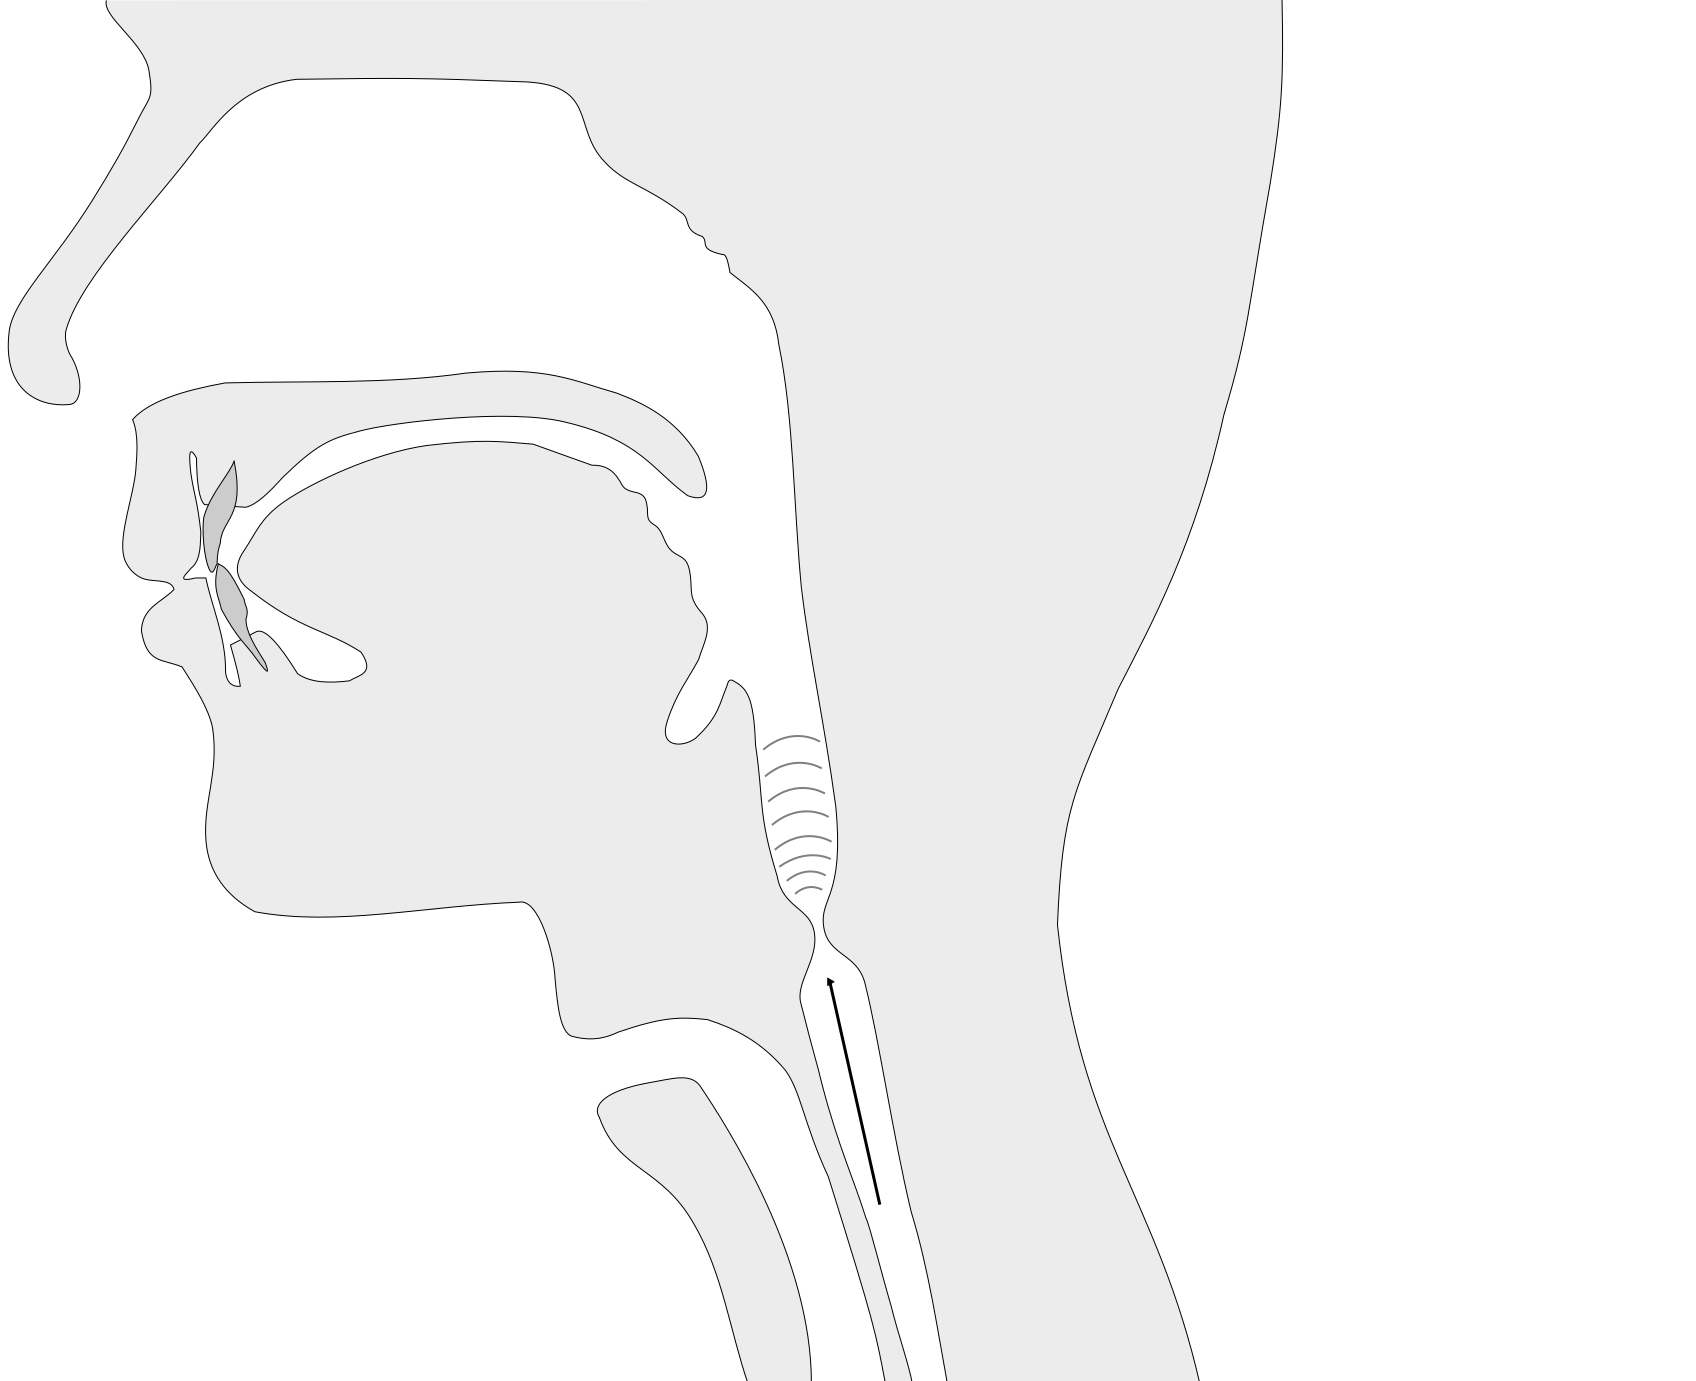
\includegraphics[width=0.6\linewidth]{ch2-cause/figures/esophageal}
    \caption[Princip tvorby jícnového hlasu]{Princip tvorby jícnového hlasu. Průchodem vzduchu přes zúžení vzniká základní tón jícnového hlasu.}
    \label{fig:cause:treatment:esophageal}
  \end{center}
\end{figure}

Kromě aspirační metody je ještě možné se setkat s metodou \textbf{injekční}.
Hlavní rozdíl spočívá v principu plnění vzduchu do jícnu. Při aspirační metodě
se využívá polykání, zatímco v tomto případě je využito kořene jazyka, kterým
je vzduch vtlačován do jícnu. Následný princip produkce hlasu je již shodný s
původní metodou. S tímto principem se můžeme setkat u pacientů, kterým byla
při laryngektomii odstraněna jazylka a aspirační náplň není možná.

Proces učení jícnového hlasu by měl začít co možná nejdříve po operaci. Pokud
je to možné, tak se s výukou začíná ještě za pobytu pacienta na ORL klinice
nebo krátce po propuštění. V první fázi se pacient učí pouze slabiky
sestávající z explosivy a souhlásky. Postupně se však přidávají slabičné
shluky, které sice nedávají smysl, ale pomáhají v osvojení potřebné techniky.
V případě úspěšného zvládnutí se přistupuje k nácviku frází a souvislé řeči.
Potřebnou dobu k nácviku jícnového hlasu nelze přesně určit, protože je
závislá na mnoha faktorech. V literatuře se uvádí, že je potřeba 30 až 50
hodin velmi intenzivního tréninku k osvojení jícnového hlasu.

Míra úspěšnosti nácviku srozumitelného hlasu se uvádí v rozsahu od 14\% do
75\%. Takto obrovský rozsah značí o mnoha faktorech, které mohou ovlivnit
úspěšné osvojení jícnového hlasu. Mezi možné příčiny neúspěchu patří
fyziologické nebo anatomické problémy, psychologické problémy, nebo jednoduše
neadekvátní podpora při řečové terapii \cite{Brown2003}. Velkou roli také
hraje snaha a odhodlání samotného pacienta.

Nepopíratelnou výhodou této techniky rehabilitace je nezávislost pacienta na
lékaři po úspěšném osvojení jícnového hlasu a permanentní oddělení dýchacích a
polykacích cest bez rizika vniknutí potravy do dýchacích cest. Mezi nesporné
výhody také patří volné ruce při vytváření řeči. Za nevýhody se obecně
považuje srozumitelnost produkovaného hlasu. Je to způsobeno jednak
\uv{břišním} zabarvením, které je už z podstaty metody přítomné, a dále také
nízkou intenzitou a krátkou výdrží při tvorbě tónu. Za negativum se dá také
považovat množství pacientem vynaloženého úsilí potřebného k osvojení
techniky. Velmi často se také mluvčí ostýchají jícnový hlas používat, protože
mají pocit, že je společensky nevhodné dorozumívat se formou blízkou říhání. Z
tohoto důvodu se odhaduje, že v běžném životě využívá jícnový hlas pouze 20 až
30\% pacientů, kteří se začali tuto techniku učit \cite{Hradecka2007}.

% subsubsection jícnový_hlas (end)

\subsubsection{Elektrolarynx} % (fold)
\label{ssub:cause:treatment:foniatric:elektrolarynx}

Rehabilitace hlasu pomocí elektrolarynxu se řadí mezi tzv. elektromechanické
metody. Princip spočívá v přikládání zařízení, které obsahuje generátor zvuku
nazývaný elektrolarynx. Přiložením do oblasti spodiny úst a aktivací zařízení
se generovaný zvuk a vibrace přenášejí do dutiny ústní a dalších přilehlých
artikulačních orgánů. Následnou artikulací je pacient schopen hovořit.
Znázorněno na obr. \ref{fig:cause:treatment:electrolarynx}.

\begin{figure}[htb]
  \begin{center}
    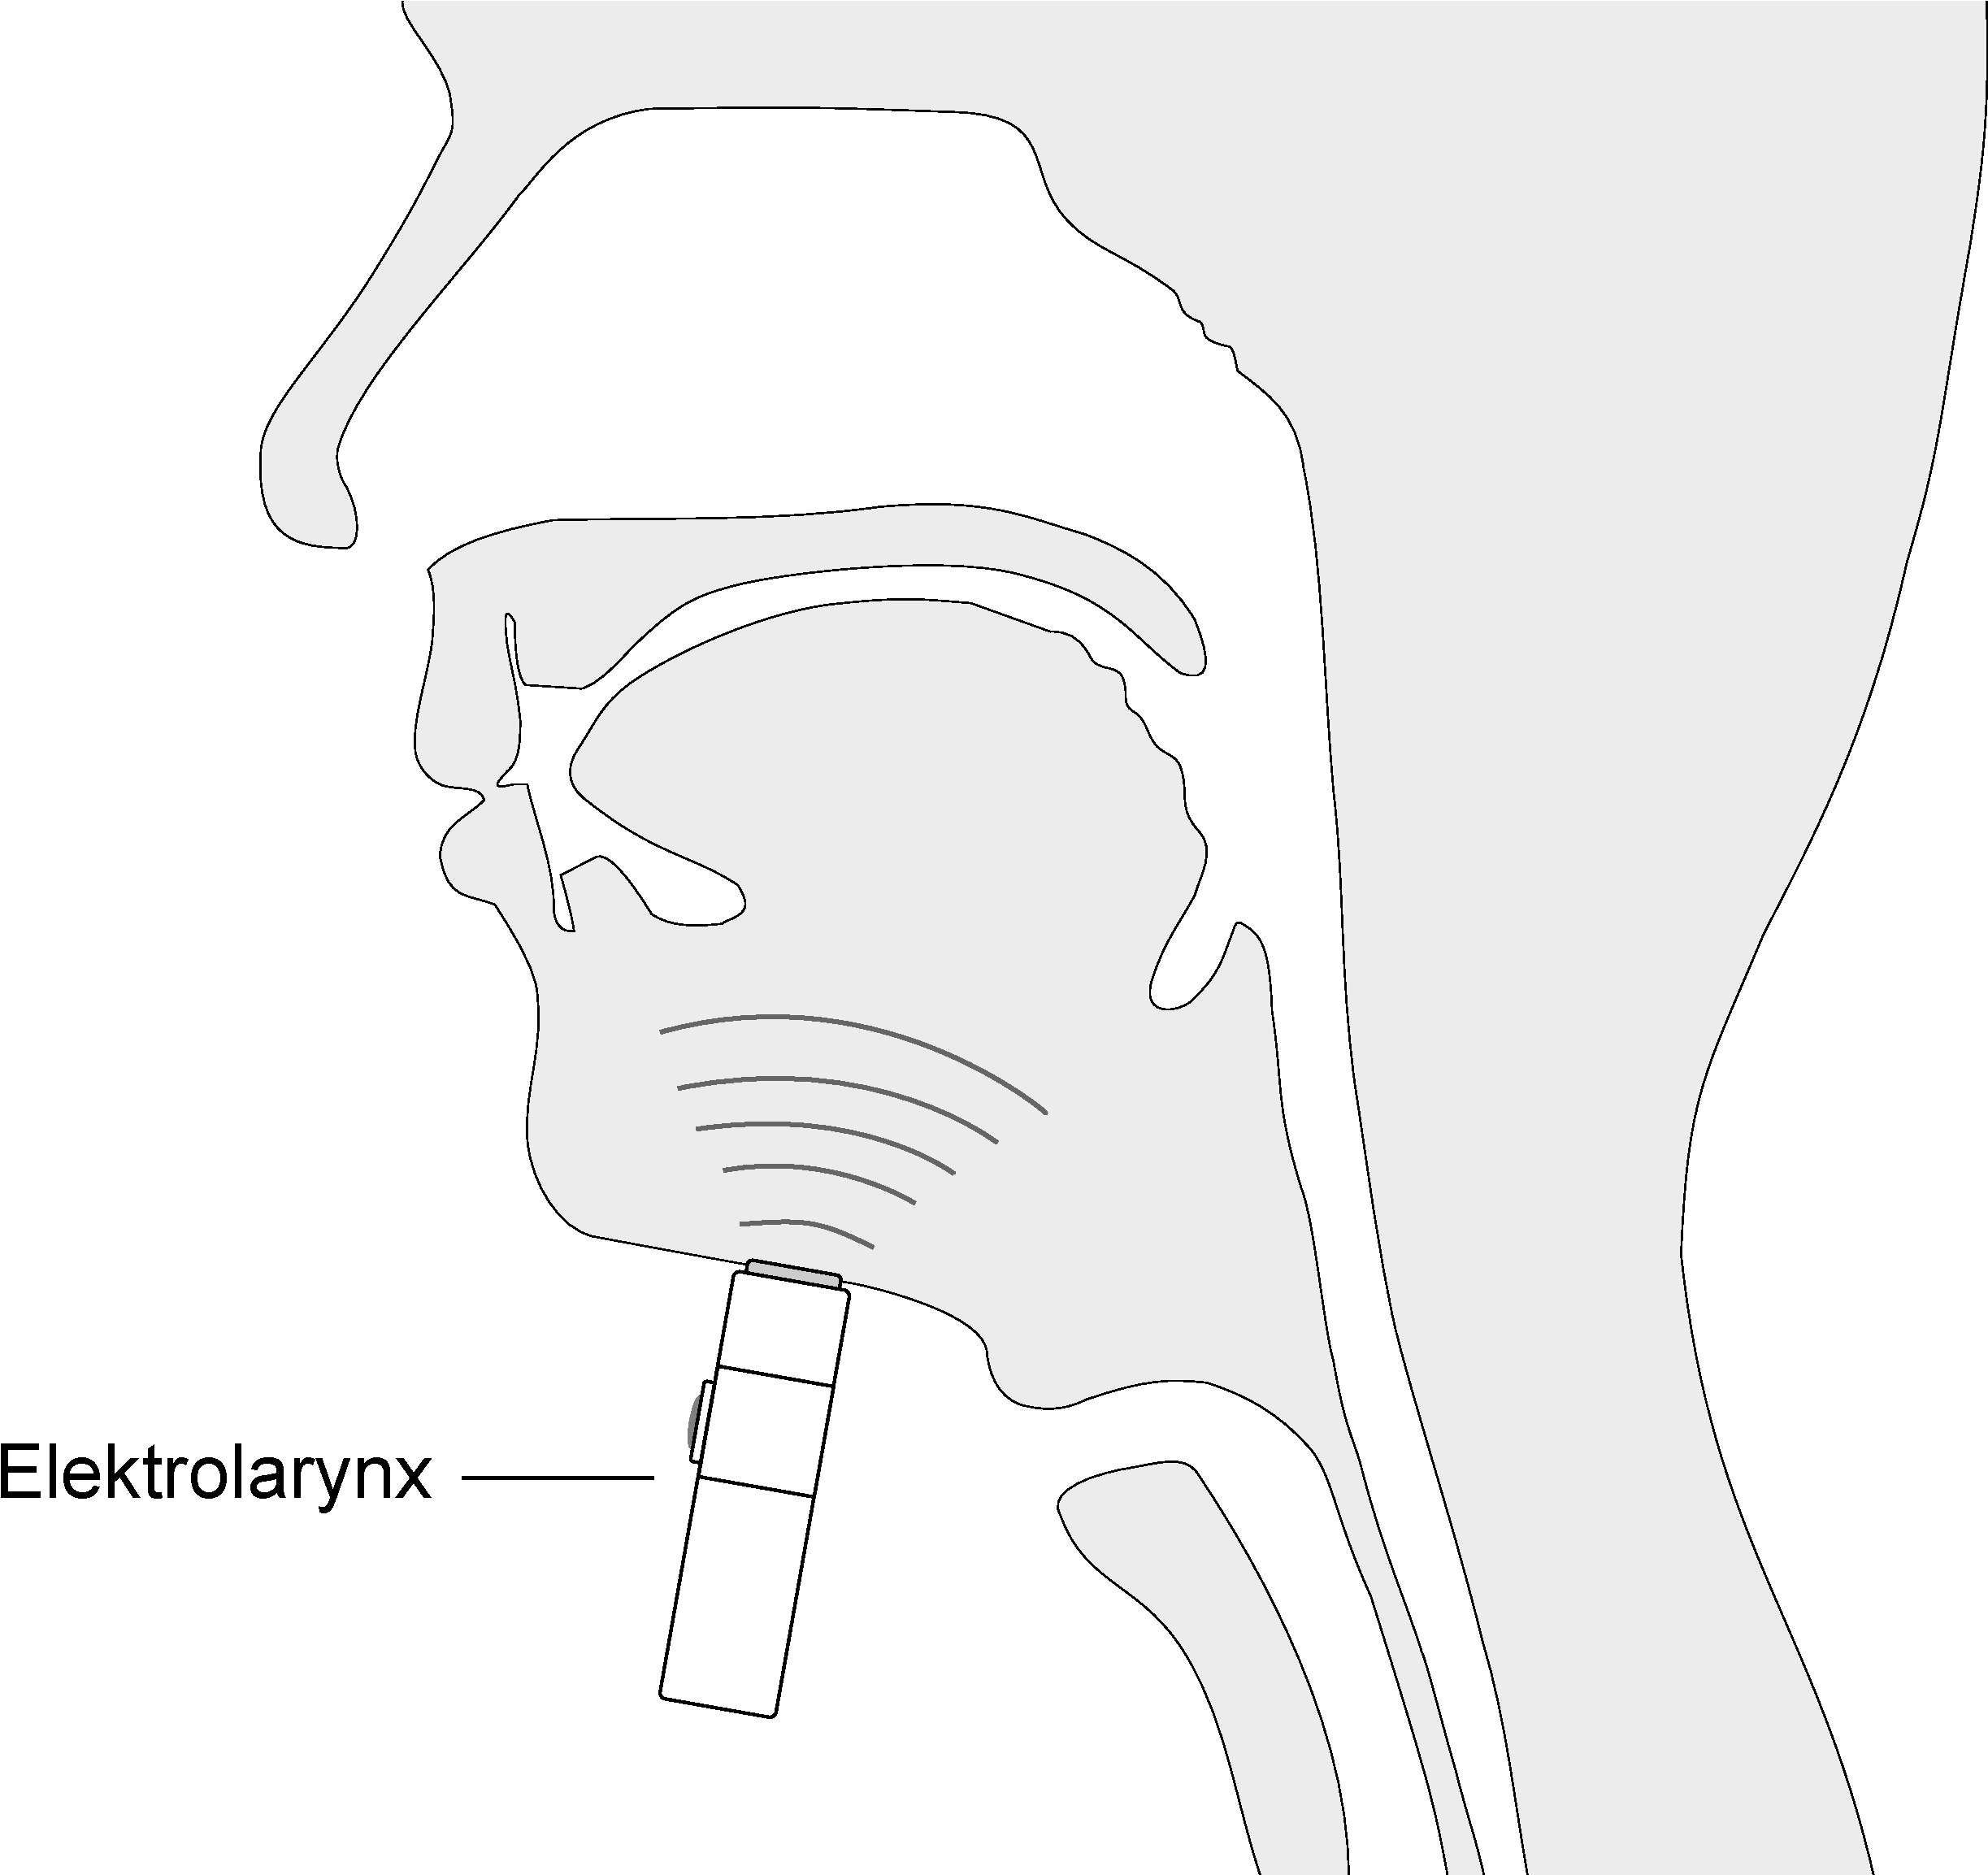
\includegraphics[width=0.6\linewidth]{ch2-cause/figures/electrolarynx}
    \caption[Princip rehabilitace hlasu pomocí elektrolarynxu]{Princip rehabilitace hlasu pomocí elektrolarynxu.}
    \label{fig:cause:treatment:electrolarynx}
  \end{center}
\end{figure}

% TODO: ELEKTROLARYNX pasaze o monotonosti reci poradne promyslet

Takto generovaná řeč se vyznačuje několika charakteristickými rysy. V první
řadě řeč budí velmi mechanický dojem. Důvodem je samozřejmě samotný
elektrolarynx, jelikož se jedná o elektromechanický generátor zvuku s
konstantním buzením, je také základní frekvence produkovaného hlasu více či
méně konstantní. Řečník tak má velmi omezené možnosti, jak řeč emotivně
zabarvovat. V průběhu času se objevily snahy průběžně měnit frekvenci zařízení
a tím ovlivňovat základní frekvenci produkované řeči \cite{Kikuchi2004,
Uemi1994, Goldstein2004}. Hlavním problém všech těchto zařízení je docílit
změnu fundamentální frekvence na základě toho, co chce řečník říci. V současné
době existují pouze experimentální zařízení, která umožňují ve velmi omezené
míře změnu frekvence \cite{Liu2007}. Další charakteristický rys představuje
nižší srozumitelnost řeči, která se ještě snižuje s~rostoucím okolním hlukem.
Velmi často se stává, že posluchač, který se s takto produkovanou řečí setkává
poprvé, není schopen plně porozumět. Se srozumitelností souvisí i další
charakteristický rys, kterým je přítomnost zvukového podkresu produkovaného
samotným přístrojem.

Za hlavní výhodu elektrolarynxu se považuje rychlost osvojení schopnosti
produkovat řeč. Zároveň je tato metoda vhodná pro téměř všechny pacienty
postižené ztrátou hlasu způsobenou léčbou karcinomu hrtanu. Z tohoto důvodu se
hojně užívá u pacientů, kteří si neosvojili jícnový hlas nebo u nich není
možné využití ostatních chirurgických metod.
Za nevýhody se obecně pokládá kvalita produkované řeči, tedy monotonní a
mechanicky znějící hlas. Dále potom zaměstnání jedné ruky držením nebo
spouštěním zařízení.

Samostatnou kapitolou může být psychologický dopad na pacienta. Stejně jako
u~jícnového hlasu se řeč produkovaná promocí elektrolarynxu jeví odlišně od
řeči přirozené. Navíc se ještě přidává potřeba využití nějakého zařízení.
Člověk proto v~mnoha případech cítí ostych a bojí se na veřejnosti mluvit.

% subsubsection elektrolarynx (end)

% subsection subsection_name (end)

\subsection{Chirurgicko-protetická metoda} % (fold)
\label{sub:cause:treatment:tracheo}

Další možnost rehabilitace hlasu představuje tracheoezofageální (zkr. TE) protéza.
První zmínka o vytvoření fistule\footnote{fistule (česky píštěl) je abnormální
otvor mezi dvěma dutými orgány, nebo mezi dutým orgánem a kůží.} mezi
průdušnicí a jícnem pochází z roku 1932. V~tomto roce doktor Guttman poprvé
vytvořil tracheoezofageání shunt\footnote{shunt - kanál, kterým je tekutina
odkloněna z přirozené dráhy. Tento kanál může být vytvořen chirurgicky nebo
pomocí syntetické trubice.} (\uv{umělá píštěl}). Hlavní myšlenka spočívá ve
vytvoření cesty prostřednictvím píštěle, pomocí které u tracheostomovaného
člověka může proudit vzduch z plic do úst. Za normálních okolností vzduch
proudí skrze tracheostomii a do úst se tak nedostane. Zacpe-li si pacient
stomu, může proud vzduchu proudit skrze píštěl do úst. Vzduch procházející
přes fistuli naráží do stěn jícnu a je rozvibrován. Tyto vibrace jsou následně
modulovány pomocí artikulačních ústrojí a tak vzniká řeč.
Tento ojedinělý zákrok otevřel cestu k chirurgické hlasové rehabilitaci.
Vzniklo několik operačních metod, které se navzájem lišili víceméně jen
umístěním fistule \cite{Kramp2009}.

Hlavní snahou chirurgů bylo vytvoření bezpečné, správně nasměrované píštěle
umožňující tvorbu hlasu. Bohužel v mnoha případech byly tyto zákroky spojené
s~vážnými komplikacemi (infekce, zápaly či těžká krvácení). Důležitým
problémem, se kterým se jednotlivý tvůrci museli vypořádat, byla stálost
vytvořeného otvoru tak, aby jím neprotékaly tekutiny špatným směrem a
nedocházelo k zatékání do dýchacích cest a orgánů. Jelikož se jednalo o velmi
náročné techniky, a bylo s nimi spojeno velké množství rizik, došlo v
80.letech 20.století k opadnutí snah tyto metody aplikovat.

Svou renesanci zažily s vložením jednocestného ventilu, který umožňoval pouze
jednosměrný průchod tekutin skrze píštěl, jak je ilustrováno na obr.
\ref{fig:cause:treatment:shunt}. První komerčně dostupná protéza se objevila
v~80.letech 20.století v USA. Na obr. \ref{fig:cause:treatment:prosthesis} jsou
zobrazeny příklady různých typů protéz. Na používané protézy jsou kladené
přísné nároky a musí vyhovovat určitým požadavkům. Předně se musí vyrábět
z~biokompatibilního materiálu, který odolává biodegradaci. Tím je zaručena
dlouhodobá trvanlivost a správná funkce. Potřebný tlak k otevření
faryngoezofageálního segmentu by měl být co nejnižší, aby bylo možné vytvářet
plynulou řeč. První vyráběné protézy měly tento tlak příliš vysoký a omezovaly
tak množinu potencionálních pacientů. Nejmodernější protézy se již vyznačují
velmi nízkým otevíracím fonačním tlakem. V~neposlední řadě by měla být protéza
samofixační a snadno vyměnitelná.

\begin{figure}[htb]
  \begin{center}
    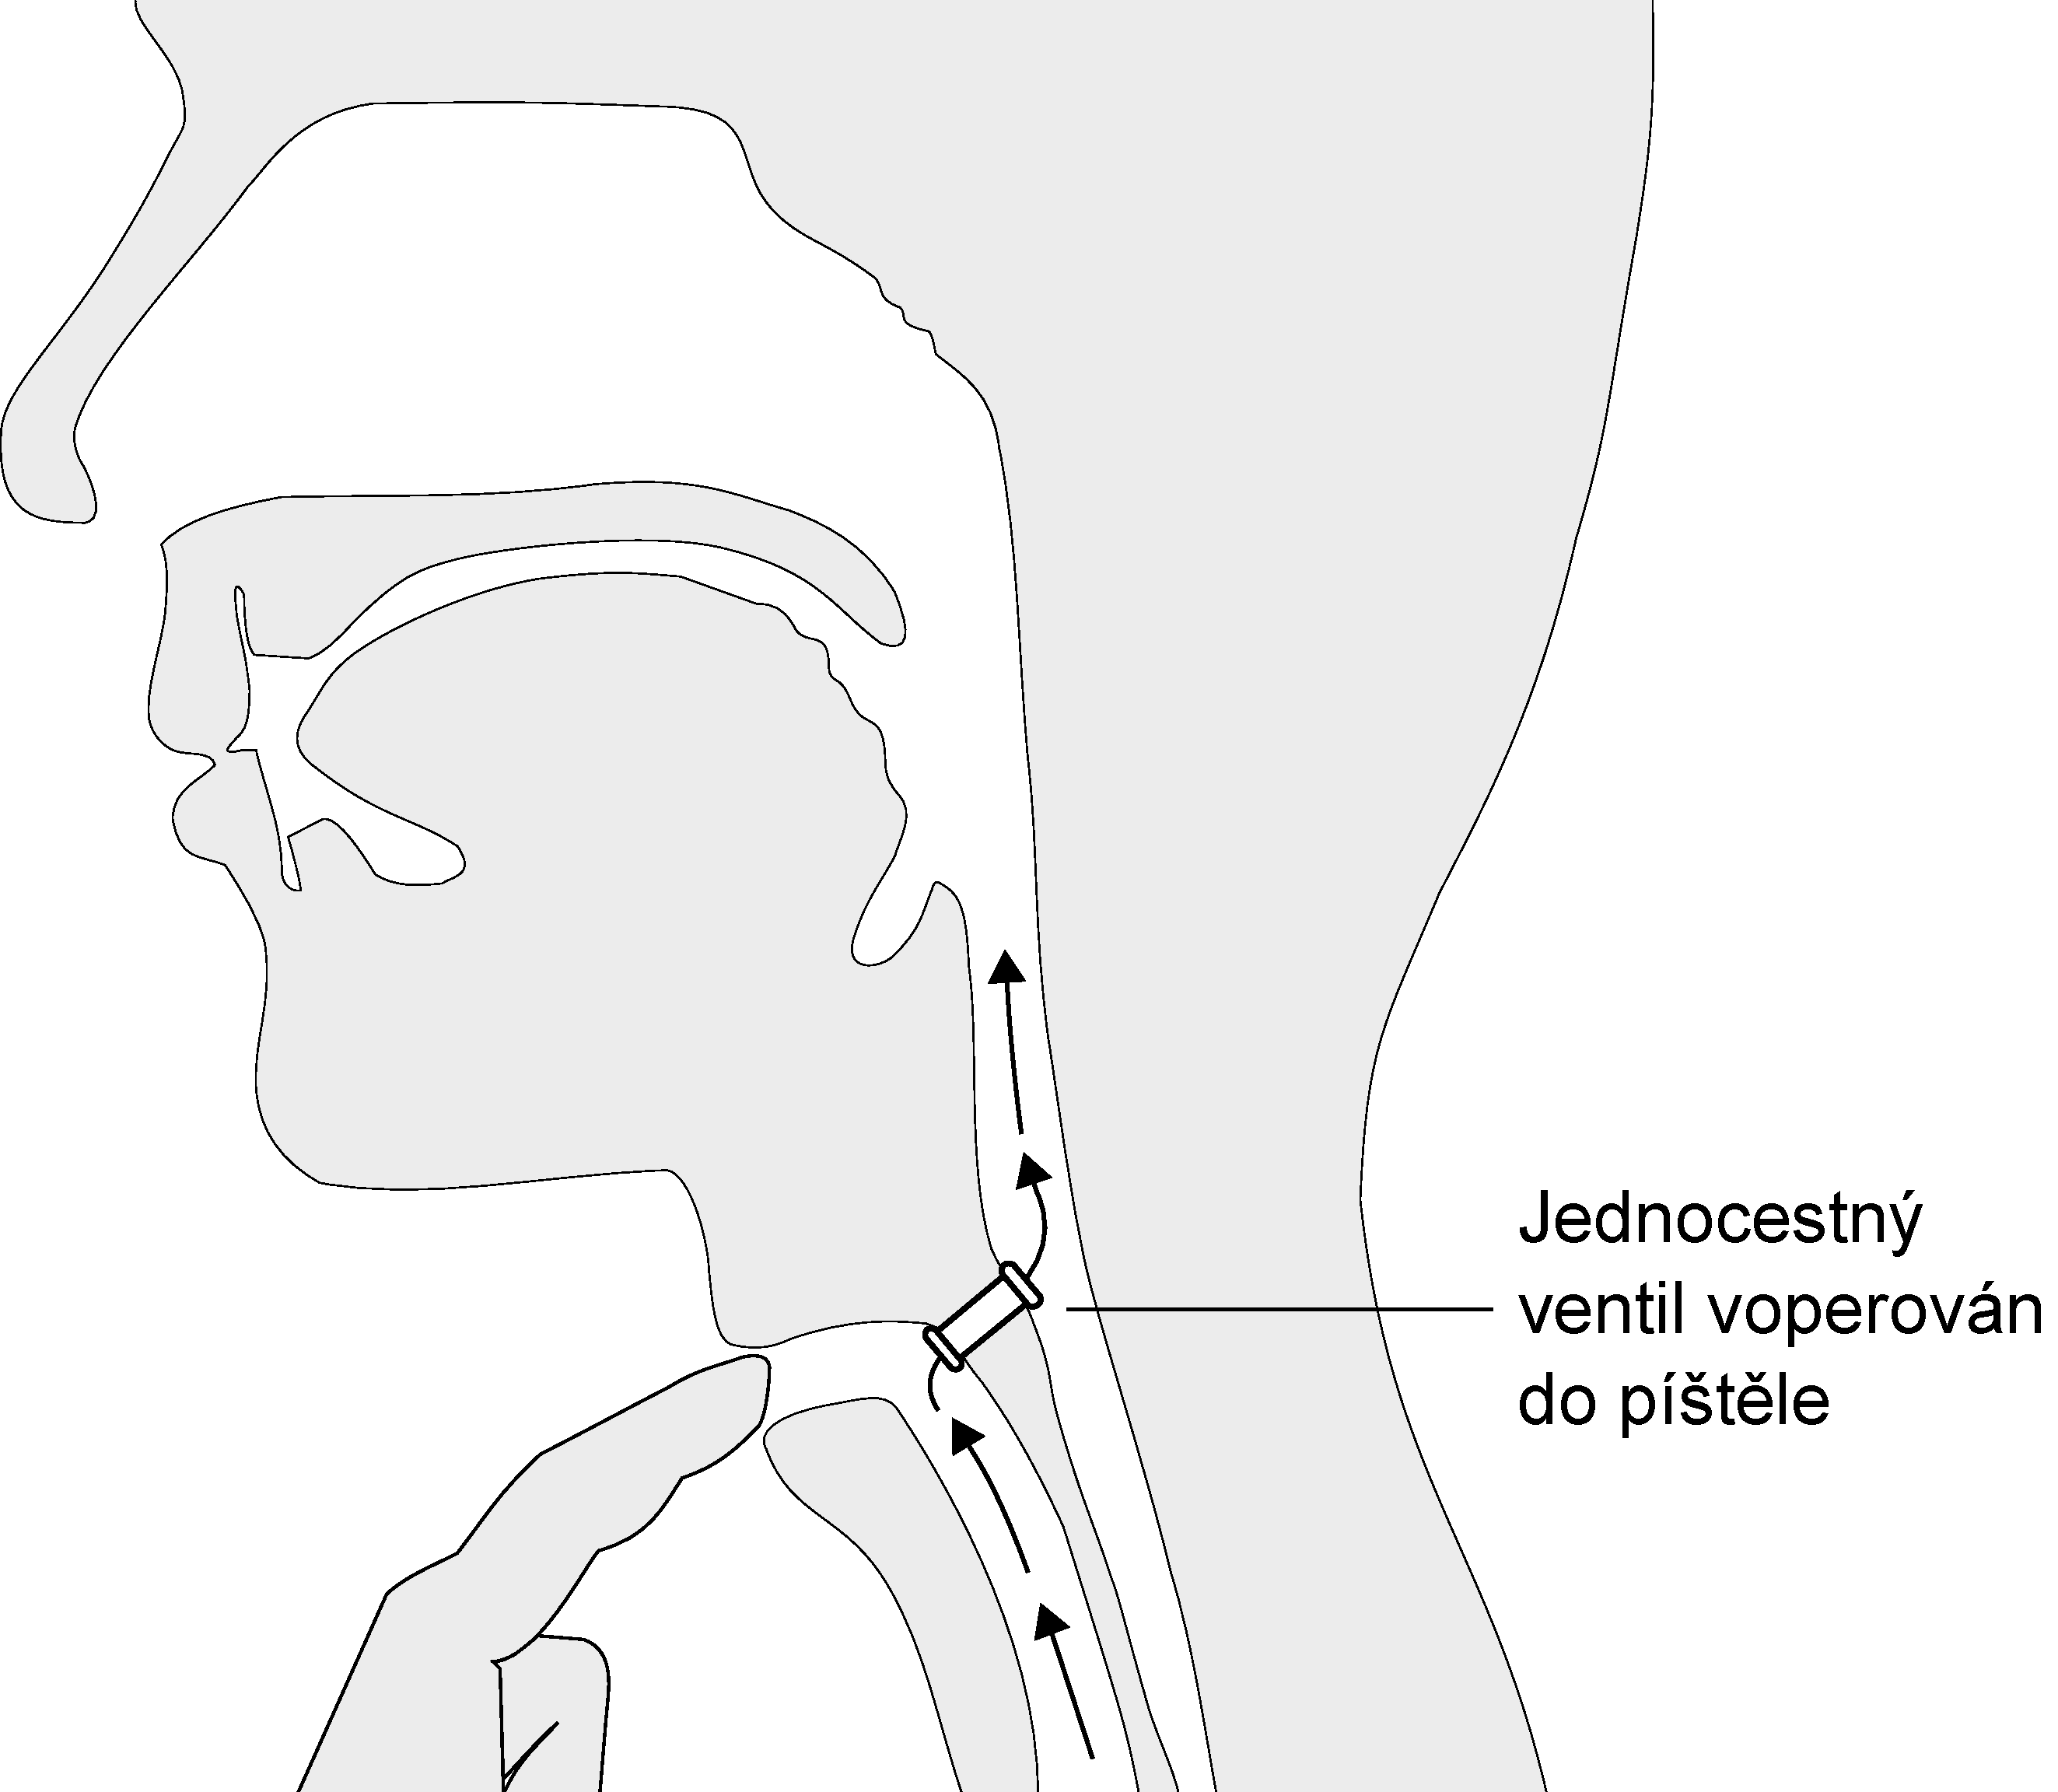
\includegraphics[width=0.6\linewidth]{ch2-cause/figures/te-shunt}
    \caption[Průchod vzduchu tracheoezofageální protézou]{Průchod vzduchu tracheoezofageální protézou.}
    \label{fig:cause:treatment:shunt}
  \end{center}
\end{figure}

\begin{figure}[htb]
  \begin{center}
    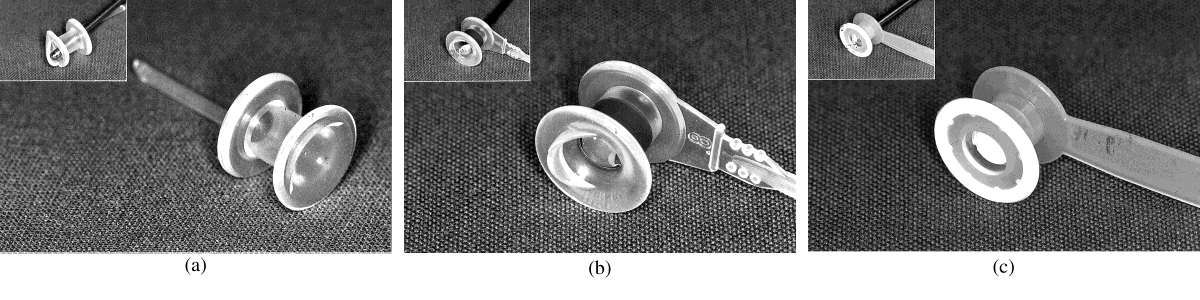
\includegraphics[width=0.9\linewidth]{ch2-cause/figures/te-protezy}
    \caption[Ilustrace používaných TE protéz]{Ilustrace používaných TE protéz (a) Gronigenova nízkotlaká protéza, (b) Provox2 a (c) Blom-Singer protéza.}
    \label{fig:cause:treatment:prosthesis}
  \end{center}
\end{figure}

V praxi se používá několik druhů protéz. Hlavním rozdílem mezi nimi však je
zda se pacient přímo účastní výměny ventilu, jehož fundamentální funkcí je
vytvoření průchodu pro vzduch proudící z průdušnice do jícnu. U protéz, které
jsou vyměňovány operačně, se doba používání pohybuje od 3 do 6 měsíců. Tento
interval velmi významně ovlivňuje tvorba biofilmu na povrchu náhrady. K tvorbě
dochází následkem přímého kontaktu protézy s tělními tekutinami a potravou.
Rychlost tvorby biofilmu ovlivňuje tvar a materiál, ze kterého je náhrada
vytvořena \cite{Leunisse2001}. U typů, které si nositel může měnit sám, se
předpokládá, že budou čištěny nebo měněny přibližně jednou za dva týdny.

Samotný zákrok zavedení protézy je možné provést zároveň s výkonem totální
laryngektomie (tzv. primární zavedení hlasové protézy) nebo až po zotavení
pacienta z~náročné léčby nádorového onemocnění (tzv. sekundární zavedení).
Primární zavedení umožňuje začít s hlasovou rehabilitací krátce po odstranění
hrtanu. Zároveň pacient nemusí v krátké době podstupovat druhou operaci, při
které by se vkládal jednocestný ventil do vytvořené fistule.

V praxi se ukázalo, že úspěšnost rehabilitace je více než 80\%
\cite{Slavicek2002}. Důležitým faktorem, stejně jako u jícnového hlasu, je
funkčnost faryngoezofageálního segmentu. Dále také otvírací tlak horního
jícnového svěrače. Hlas tvořený protézou se vyznačuje vysokou kvalitou, dobrou
srozumitelností, individuálním zabarvením a relativně dlouhou fonační dobou
dosahující průměrně 20 sekund \cite{Saito2003}. Oproti jícnovému hlasu není potřeba
tak intenzivní edukace pacienta k plnému osvojení hlasu. V současnosti se
jedná o nejpoužívanější metodu rehabilitace hlasu.

% TODO: Vyhody nevyhody metody - film tvorici se na proteze
% TODO: Kriteria na pacienta


% subsection chirurgicko_protetická_metoda (end)

\subsection{Hrtanu podobné struktury} % (fold)
\label{sub:cause:tratment:structure}

S rozvojem mikrovaskulárních\footnote{mikrovaskulární - část oběhového systému
složeného z nejmenších cév, jako jsou kapiláry, žilky aj.} transplantátů se
začaly objevovat postupy, které umožňovaly rehabilitovat hlas pouze pomocí
chirurgického zákroku. Tyto techniky umožňují permanentní spojení hypofaryngu
s tracheou pomocí vlastní tkáně pacienta.

První takovouto  metodu představil v roce 1984 doktor Ehrenberger
\cite{Kramp2009}, který popsal tzv. \uv{\textbf{řečový sifón}} (angl. \textbf{speech
siphon}). Tento sifón je vytvořen z části tenkého střeva zvané lačník
(jejunum). Spojení mezi hrtanem a hltanem je dvakrát esovitě zahnuto tak, aby
bylo minimalizováno riziko sekundární aspirace. Schéma \uv{řečového sifónu}
podle Ehrenberga je znázorněno na obr. \ref{fig:cause:treatment:microvascular}
A. Již na první pohled je zřejmé, že se jedná o velmi náročný chirurgický
zákrok. První články publikované autorským kolektivem prezentovaly velmi dobré
funkční výsledky metody. Podle \cite {Sebova-Sedenkova2006} bylo doposud
operováno přibližně 60 pacientů.

V roce 1990 byla popsána laryngoplastika podle Hagena. V tomto případě se
vytváří tzv. \textbf{neolarynx}, k jehož vytvoření se používá štěp z
předloktí. Vnitřek neolaryngu je kryt kůží. Neoglottis je vyztužen chrupavkou
a překrývá vchod do neolaryngu tak, aby nedocházelo k sekundární aspiraci.
Laryngoplastika podle Hagena je znázorněna na obr.
\ref{fig:cause:treatment:microvascular} B. Doposud bylo operováno přibližně 300
pacientů \cite{Sebova-Sedenkova2006}.

\begin{figure}[htb]
  \begin{center}
    
\includegraphics[width=0.9\linewidth]{ch2-cause/figures/microvascular}
    \caption[Schéma \uv{řečového sifónu} a laryngoplastiky]{A) Schéma \uv{řečového sifónu} tak jak jej představil Ehrenberg. B) Laryngoplastika podle Hagena}
    \label{fig:cause:treatment:microvascular}
  \end{center}
\end{figure}

Bohužel v současné době tyto metody nenacházejí širší uplatnění. Především je
to způsobeno chirurgickou náročností samotných metod, kvůli které se velmi
těžko prosazují na dalších pracovištích. Dalším aspektem, který limituje tyto
metody, je vliv na samotného pacienta. Metody předpokládají další chirurgický
zákrok vykonaný po totální laryngektomii. Tento zákrok představuje další zátěž
pro pacienta nemluvě o~možných komplikacích. I přes nedostatky těchto metod je
pochopitelná snaha lékařů o intenzivní výzkum v této oblasti. Při úspěšné
léčbě je pacient schopen produkovat hlas velmi dobré kvality a ve většině
případů nepotřebuje žádnou péči ze strany lékařů ORL.

% subsection hrtanu_podobné_struktury (end)

\subsection{Transplantace hrtanu} % (fold)
\label{sub:cause:treatment:transplantation}

Nejkomplexnější možnost rehabilitace hlasu představuje transplantace hrtanu.
V~tomto případě pacient obdrží implantovaný hrtan od dárce. Pokud je
transplantace úspěšná, přebírá transplantovaný orgán plně funkci původního
orgánu a velmi významně zvyšuje šance pacienta na plné zotavení bez trvalých
následků.

První informace spojené s výzkumem možností provedení transplantace hrtanu se
objevují již v 60. letech 20. století\footnote{Vůbec první úspěšná transplantace
orgánu (ledvin) se uskutečnila v roce 1954.}. Přesto byla první totální
hrtanová transplantace provedena až profesorem Marshallem Stromem v roce 1998
\cite{Narula2011} a do dnešních dnů byly provedeny pouze 2 kompletní
transplantace.

Prvním pacientem, který podstoupil transplantaci, byl čtyřicetiletý muž z USA.
K~laryngektomii v jeho případě vedla motocyklová nehoda, při které si pacient
rozdrtil hrtan. K incidentu došlo 20 let před transplantací. Před zákrokem
používal k~produkci řeči elektrolarynx. Dárcem orgánu byl taktéž čtyřicetiletý
muž, který zemřel na mozkové aneurysma. Úspěch transplantace se na příjemci
projevil již třetí den po operaci, kdy poprvé po 20 letech promluvil (vyslovil
anglické slovo \uv{hello}). Přibližně po 36 měsících od transplantace byl
produkovaný hlas srovnatelný s hlasem zdravého člověka. Podle vlastních slov
pacienta se po operaci jeho kvalita života \uv{nesmírně} zlepšila.
\cite{Strome2001} Doposud poslední úspěšně vykonaná transplantace byla
zaznamenána v~říjnu 2010.

Mezi hlavní důvody takto malého počtu zákroků patří množství pacientů vhodných
pro tuto proceduru. Jelikož se jedná o transplantaci dárcovského orgánu je
nutné použití imunosupresiv, tedy medikamentů zabraňující odmítnutí orgánu.
Imunosupresiva jsou však v současné době nepoužitelná u lidí trpících
rakovinou hrtanu z důvodu velmi vysokého rizika rozšíření rakoviny
\cite{Narula2011}. Další problém představuje náročnost samotného zákroku.
Předně je potřeba provést reinervaci a obnovení krevního oběhu v implantovaném
orgánu. U první provedené transplantace se nepodařilo dosáhnout kompletní
reinervace. Výsledkem tak byl velmi kvalitní generovaný hlas, ale zároveň
nebylo možné pomocí hrtanu zabezpečit bezproblémové dýchání a bylo proto nutné
ponechat tracheostomii.

Poslední výzkum v oblasti imunosuprese však naznačuje, že by v dohledné době
mohlo dojít k pokroku a umožnit transplantaci hrtanu i u lidí trpících
rozsáhlou rakovinou v oblasti krku \cite{Narula2011}. Prozatím je však tato
metoda vhodná pro pacienty netrpící rakovinou, případně ty, u kterých
převažovaly benigní nádory a již 5 let nedošlo k recidivě.

% subsection transplantace_hrtanu (end)

\subsection{Shrnutí} % (fold) \label{sub:treatment:summary}

% NOTE: Neni lepsi pouzit dusledky misto nasledky 3

Rehabilitaci pacientů, kteří prodělali chirurgické odstranění hrtanu, je ve
vyspělých zemích věnována značná pozornost, jelikož následky této operace,
oproti jiným druhům léčby, velmi významně ovlivňují kvalitu života pacientů. V
první řadě se léčený musí vyrovnat se ztrátou hlasu. Tato situace je již sama
o sobě velmi náročnou psychickou zkouškou. Ztráta hlasu je však pouze jedním z
vícero problémů, se kterými je potřeba se vypořádat. Mezi další patří možná
ztráta čichu či vyšší náchylnost k respiračním onemocněním. Neméně významnou
roli sehrává i fyzická odlišnost a z~toho pramenící psychická zátěž pacienta
po absolvované léčbě.

 V současnosti
nejpoužívanějšími metodami rehabilitace hlasu jsou \textbf{tracheoezofageální
píštěl} (popsáno v části \ref{sub:cause:treatment:tracheo}), \textbf{jícnový
hlas} (\ref{ssub:cause:treatment:foniatric:esophageal}) a použití
\textbf{elektrolarynxu} (\ref{ssub:cause:treatment:foniatric:elektrolarynx}).
Existují samozřejmě i další a přehled v současnosti používaných je uveden
v~tab. \ref{tab:treatment:summary}.

\newcolumntype{b}{X}
\newcolumntype{s}{>{\hsize=.5\hsize}X}

\begin{table}[ht]
  \centering
  \begin{tabularx}{1.0\textwidth}{L{1.2} L{0.6} L{1.1} L{1.1}}
    & \textbf{Kvalita} & \textbf{Výhody} & \textbf{Nevýhody} \\
    \toprule \\ [-1.75ex]

    \textbf{Tracheoezofageální píštěl} & Vysoká & Vysoká míra osvojení, dlouhá fonační doba & Zanášení píštěle a s ním spojené čištění, případně dodatečná lékařská péče \\
    \midrule \\ [-1.75ex]

    \textbf{Jícnový hlas} & Dobrá & Volné ruce při mluvení, není potřeba dodatečné lékařské péče & Velmi náročná metoda k naučení, nepřirozený hlas \\
    \midrule \\ [-1.75ex]

    \textbf{Elektrolarynx} & Nízká & Snadné k naučení & Monotonní až robotický hlas, nutné nosit externí elektrické zařízení \\
    \midrule \\ [-1.75ex]

    \textbf{Hrtanu podobné struktury} & Vysoká & Nezávislost pacienta na pravidelné lékařské péči & Velmi náročná chirurgická procedura, která pacienta vystavuje dalším možným rizikům  \\
    \midrule \\ [-1.75ex]

    \textbf{Transplantace hrtanu} & Velmi vysoká & Transplantovaný hrtan přejímá funkci odstraněného orgánu & Velmi náročná chirurgická procedura, která je vhodná jen pro malé procento pacientů \\
  \end{tabularx}

  \caption{Přehled dostupných metod rehabilitace hlasu \label{tab:treatment:summary}}
\end{table}

Většina pacientů je tedy rehabilitována pomocí tracheoezofageálního píštěle,
který principiálně vychází z jícnového hlasu, jehož negativa se snaží
eliminovat. O úspěchu rehabilitace, stejně jako u jícnového hlasu, tak
především rozhodují vlastnosti faryngoezofageálního segmentu. Pokud pacient
není schopen si osvojit jícnový hlas, případně nemá voperován píštěl, je
použit elektrolarynx. Bohužel tyto metody neřeší další problémy spojené s
odstraněním hrtanu, a proto se lékaři stále snaží zdokonalovat rehabilitační
metody. Za nejkomplexnější se dá považovat úplná transplantace hrtanu, která
řeší víceméně všechny problémy spojené s odstraněním hrtanu. Bohužel tento
zákrok je velmi náročný a vhodný pouze pro malou část pacientů.
I když je tedy v současné době lékařská věda schopna rehabilitovat hlas, tak
zde zůstává otevřený prostor pro inovace a tím zlepšení kvality života lidí
postižených ztrátou hrtanu.

% subsection treatment:summary (end)

% section rehabilitace_hlasu_po_totalni_laryngektomii (end)

